
\chapter*{Реферат}
\addcontentsline{toc}{chapter}{Реферат} 
\renewcommand{\thefigure}{\arabic{figure}} % Plain numbering
\setcounter{figure}{0}                     % Reset if needed

\begin{center}
    Общая характеристика диссертации
\end{center}

\section*{Актуальность темы}
Квантовое распределения ключа (КРК) - актуальная технология, появившаяся из теории квантовой информатики, позволяющая распределить симметричную битовую последовательность с помощью квантовых методов у двух и более пользователей для использования этой последовательности в качестве ключа для симметричного шифрования данных и одновременным обнаружением несанкционированного доступа со стороны нелегитимных пользователей. Использование квантовых состояний света при распределении ключа позволяет достичь уровня секретности, недоступного для классических протоколов шифрования. Такие квантовые состояния могут быть представлены в виде одиночных фотонов. Их квантовые свойства не позволяют злоумышленнику скопировать их состояния или считать их без изменения и без внесения ошибок. Такие квантовые состояния возможно передавать как по волоконно-оптическим линиям связи (ВОЛС), как по атмосферным каналам, так и в космическом пространстве с помощью спутников. Принцип работы данных систем следующий. На стороне передатчика (Алиса) формируются квантовые состояния. Для этого используется когерентное лазерное излучение, ослабленное до одиночных фотонов с помощью аттенюатора. В подготовленные кванты света вносится изменение в поляризацию или фазовый сдвиг фотона. Подготовленное таким образом состояние передается по каналу связи к приемнику (Боб). На приемной стороне происходит независимое от Алисы повторное измерение состояния фотона. В случае корреляции у Боба принятый одиночный фотон регистрируется детектором одиночных фотонов. Благодаря свойствам одиночного фотона в виде невозможности клонирования, невозможности измерения без разрушения и его неделимости возможно отследить воздействие злоумышленника, так как его действия будут приводить к появлению ошибок в полученной битовой последовательности. Так обеспечивается контроль несанкционированного допуска. 

Отдельным классом выделяются системы квантового распределения ключа на непрерывных переменных (КРК-НП). В таких системах квантовое состояние, подготовленное и переданное Алисой, на приемной стороне взаимодействует с сильным лазерным излучением. И результат этого взаимодействия регистрируется балансным детектором. Основными отличиями данного детектора от детектора одиночных фотонов является использование двух классических фотоприемников, подключенных таким образом, что их фототоки взаимно вычитаются, что позволяет уменьшить шум системы, и отсутствие охлаждения до температур порядка -40$^{\circ}$  градусов Цельсия. Все это позволяет упростить конечную систему. К преимуществам КРК-НП можно отнести большую скорость выработки секретного ключа по сравнению с системами КРК на дискретных переменных, в которых применяются детекторы одиночных фотонов. 

Среди сложностей систем КРК-НП выделяется способ передачи сильного лазерного излучения или локального осциллятора (ЛО) на приемную сторону и его разделения с квантовым сигналом. В первых системах КРК-НП с Гауссовой модуляцией Локальный осциллятор и квантовые состояния генерировались у передатчика, объединялись и передавались совместно в квантовый канал. На приемной стороне локальный осциллятор и квантовый сигнал разделяются, ЛО задерживается специальной линией задержки и снова соединяются на светоделителе для взаимодействия. Результатом этого взаимодействия является интерференционная картина, распределение интенсивности которой зависит от закодированного Алисой состояния. Полученное поле регистрируется балансным детектором, на выходе такого формируется уровень напряжения, который в дальнейшем подвергается пост-обработке.  Передача локального осциллятора через канал ограничивает дальность работы системы такого типа и ограничивает скорость выработки ключа, так как для лучшей работы системы необходим ЛО как можно большей мощности. Второй проблемой является возможности злоумышленника манипулировать локальным осциллятором для создания каналов утечки информации. В качестве альтернативы предлагается использовать локальный осциллятор, сгенерированный на приемной стороне. Такое решение позволит увеличить дальность передачи ключа, скорость его выработки и закрыть уязвимость к атаке на ЛО.


Одним из перспективных подходов к реализации систем квантовой коммуникации на непрерывных переменных является система квантовой коммуникации на боковых частотах модулированного излучения. В основе данного метода лежит вынесение квантового канала на боковые частоты, которые появляются в результате модуляции оптического излучения переменным электрическим полем. Благодаря этому повышается устойчивость передаваемого сигнала ко внешним воздействиям и обеспечивается высокая спектральная эффективность, а также обеспечивается показатели по отношению скорости выработки ключа к дальности между блоками приемника и передатчика, сравнимые с другими системами квантовой коммуникации. Данный метод подходит и для реализации протоколов на непрерывных переменных с когерентными методами детектирования. В частности, в данной работе рассматривается гетеродинный метод, при котором квантовые состояния, подготовленные Алисой, передаются по волоконной линии связи к приемнику, в нем попадают на светоделитель с формулой 2х2 и коэффициентом деления 50:50 и смешиваются на нем с мощным локальным осциллятором, который отстроен по частоте от передающего лазера на величину, которая превышает частоту смены состояний. Результат интерференции регистрируется балансным детектором. На выходе балансного детектора формируется сигнал на промежуточной частоте от всего спектра сигнала, переданного Алисой. Для извлечения информации требуется провести фильтрацию с помощью фильтра низких частот и демодуляцию полученного сигнала для генерации сырого ключа. 

Одной из проблем при реализации гетеродинного метода детектирования для распределения ключа является необходимость компенсации фазовых шумов. Для этого применяют различные методы. Первым из таких методов является передача "пилотного" импульса, при детектировании которого измеряется фазовый шум, внесенный каналом. После этого измеренное значение учитывается в постобработке состояний. Второе - это реализация обратной связи в различных формах. В рамках данной работы предлагается использовать метод оптической обратной связи для системы квантового распределения ключа на боковых частотах на непрерывных переменных. Суть данного метода заключается в инжекции лазерного излучения от ведущего лазера, который является лазером передатчика, в лазер ведомый, который используется в качестве локального осциллятора в приемнике. Данный метод позволяет стабилизировать длину волны ЛО и уменьшить фазовые шумы из-за того, что оба источника являются генераторами когерентного излучения со случайной фазой.

Метод оптической инжекции требует дополнительного канала для передачи создания обратной связи. Такой канал усложняет систему и повышает требования к волоконно-оптической линии связи (ВОЛС), что особенно критично в городских линиях связи, где выделение дополнительного волокна или канала в сетях с мультиплексированием затруднительно. Решением данной проблемы может является система квантового распределения ключа на непрерывных переменных с применением гетеродинного детектирования с независимым ЛО. Суть данной системы заключается в том, что на приемнике и передатчике установлены лазеры со стабилизацией длины волны и со шириной спектральной линии менее 10 кГц. Такой подход позволяет не прибегать к постоянной подстройке длин волн лазеров и уменьшить фазовый шум, связанный с независимостью источников излучения.
Однако, фазовый шум при этом не исчезает, поэтому его все еще необходимо компенсировать. В случае реализации такого метода детектирования сигналов для протокола квантового распределения ключа на боковых частотах для этого можно использовать несущую частоту, измеряя ее фазу и внося корректировки в постобработке. 

Отличия реальных систем КРК от моделей, используемых для теоретических доказательств, могут быть использованы злоумышленником для проведения различных типов атак на оборудование, входящее в состав системы. В работах ранее было показано, что источники лазерного излучения на основе полупроводниковых кристаллов могут быть уязвимы к "засеву" внешним излучением злоумышленника на длине волны близкой к той, что использует передатчик. В результате этой атаки изменяется форма излучаемого импульса и увеличивается выходная мощность, в отдельных случаях можно наблюдать и изменение длины волны. Эти эффекты приводят к увеличению среднего числа фотонов, излучаемых передатчиком, что открывает возможность для злоумышленника атаки с расщеплением числа фотонов. 

Однако в литературе не рассматривались атака "засевом" лазерным излучением на других длинах волн. Атака такого типа опаснее тем, что для защиты от нее используются пассивные волоконно-оптические элементы, вносящие дополнительное затухание, например, изоляторы или DWDM фильтры. Но существуют работы, которые демонстрируют, что величина затухания в таких элементах может уменьшаться при существенном изменении падающей длины волны излучения. Например, изолятор с рабочей длиной волны 1550 нм вносит 50 дБ потерь при обратном прохождении, когда при облучении излучением на длине волны 1310 нм эта величина составляет 20 дБ. А в случае с DWDM фильтром, он практически не вносит затухание на длине волны 1310 нм. Таким образом, злоумышленнику гораздо проще осуществить атаку "засевом" лазерным излучением, так как на данной длине волны вносимое затухание меньше. 

Такой тип атаки носит название "атака оптической накачкой". Ее суть заключается в том, что злоумышленник зондирует лазер длиной волны, отличной от рабочей. При этом это излучение поглощается активной средой лазера передатчика так, что поглощенное излучение выступает в роли оптической накачки, которая работает как дополнение к электрической накачки полупроводникового лазера. В этом случае изменяется Ватт-Амперная характеристика лазера и его квантовая эффективность. Это приводит к тому, что изменяется энергия излученных импульсов увеличивается при неизменной величине тока накачки. В рамках данной работы впервые обозначен данный тип атаки, определена нижняя граница необходимой мощности излучения на длине волны 1310 нм для изменения характеристик изучаемого лазера и измерено влияние оптической накачки на характеристики лазера. 

В системах квантового распределения применяются источники лазерного излучения на основе оптической инжекции. Такие источники построены следующим образом: применяются два лазера - ведущий и ведомый, соединенных циркуляторном. Излучение ведомого лазера позволяет снизить дрожание излучаемых импульсов, стабилизировать мощность выходного излучения и сузить спектральную линию. Однако такие источники не исследовались на устойчивость ко внешнему излучению. Ранее показанные работы по лазерному "засеву" были проведены только для одиночных источников излучения. Источник, построенный на основе оптической инжекции, имеет несколько преимуществ относительного одиночного: наличие изоляции от квантового канала за счет оптического циркулятора и наличие внешнего излучения ведущего лазера. В рамках данной работы изучается влияние мощного лазерного излучения на длительность, дрожание и амплитуду излучаемых импульсов, продемонстрирована нижняя граница мощности излучения необходимого  для внесения изменений в работу данной системы.
\section*{Цель}
Разработать систему гетеродинного приема сигналов в квантовой системе коммуникаций на боковых частотах с локальным осциллятором на стороне получателя с применением оптической инжекции и исследовать устойчивость к атакам на техническую реализацию источников лазерного излучения в этой системе. 

\section*{Задачи}
\textbf{Задача 1}\\
Реализация обратной связи в виде оптической инжекции для системы КРК на боковых частотах с гетеродинным методом детектирования и применением непрерывных переменных. 

\textbf{Задача 2}\\
Применение гетеродинного приема сигналов в системах КРК, и гетеродинное детектирование мультиплексированного сигнала на одной несущей\\

\textbf{Задача 3}\\
Исследовать атаку оптической накачкой на источники излучения, которые могут являться локальным осциллятором для систем квантового распределения ключа на непрерывных переменных\\

\textbf{Задача 4}\\
Исследовать влияние мощного оптического излучения на источник излучения на основе оптической инжекции\\

\section*{Основные положения, выносимые на защиту}
\begin{enumerate}
    \item Передача фазово-кодированных сигналов в системе квантового распределения ключей на непрерывных переменных с гетеродинным методом детектирования сигналов и локальным осциллятором, реализованным на стороне приемника, становится возможной при стабилизации длин волн используемых источников излучения за счет применения метода оптической инжекции для реализации обратной связи.
    \item Алгоритм, заключающийся в контроле поляризации входящего сигнала,  основанный на анализе спектрального состава электрического сигнала, полученного после Быстрого Преобразования Фурье, и с поворотом поляризации на основе проведенного анализа, позволяет произвести обмен фазово-кодированными состояниями в системе квантовой коммуникации на боковых частотах с применением непрерывных переменных и гетеродинным методом регистрации сигналов на основе двух независимых источников лазерного  излучения телекоммуникационного диапазона длин волн  и с применением частотного мультиплексирования на одной несущей частоте. 
    \item Поглощение излучения лазера нарушителя  активной средой полупроводникового лазера с распределенной обратной связью, используемого в передатчике системы квантового распределения ключей, приводит к увеличению излучаемого им среднего числа фотонов.
    \item Засеивание ведомого лазера в источнике излучения, построенного  на основе метода оптической инжекции, лазером нарушителя, который работает в непрерывном режиме, мощностью не менее 800 мВт и на длине волны, согласованной с длиной волны ведомого лазера,  повышает стандартное отклонение амплитуды выходных импульсов ведомого лазера на $3\%$, повышает стандартное отклонение их энергии на $3\%$, увеличивает стандартное отклонение длительности импульсов на $2.5\%$ и увеличивает среднюю излучаемую мощность на $8\%$, приводящее к снижению дальности передачи секретного ключа на $10\%$.
\end{enumerate}
\section*{Научная новизна}
Впервые реализована система обратной связи с помощью оптической инжекции для системы квантового распределения ключей на боковых частотах и передан просеянный ключ. Реализован гетеродинный метод детектирования сигналов с двумя независимыми источниками излучения для системы квантового распределения ключей на боковых частотах и разработан алгоритм контроля поляризации для этой системы. Впервые продемонстрирован новый тип атаки на техническую реализацию - атака оптической накачкой на источник излучения в системах квантового распределения ключей, которая позволяет увеличить излучаемое среднее число фотонов в обход существующих методов защиты. Определено экспериментально влияние мощного лазерного излучения на источник когерентного излучения на основе оптической инжекции, увеличивающее энергию излучаемых импульсов и ее разброс, увеличивает выходную мощность атакуемого источника, что в совокупности приводит к снижению скорости выработки секретного ключа.
%В работе проводились исследования по реализации новых подходов к регистрации сигналов для системы квантового распределения ключей на боковых частотах и исследовались атаки на техническую реализацию данной системы. В результате чего получены новые практические результаты, научная новизна которых заключается в том, что\\
%\textbf{Научная новизна 1}
%Разработан метод гетеродинного детектирования сигналов для системы квантового распределения ключей на боковых частотах с использованием непрерывных переменных на основе двух независимых источников излучения и алгоритм контроля поляризации этих источников лазерного излучения.\\
%\textbf{Научная новизна 2}
%Разработан метод гетеродинного детектирования сигналов с применением оптической инжекции для системы квантового распределения ключей на боковых частотах и сформирован протокол распределения секретных бит.\\
%\textbf{Научная новизна 3}
%Впервые проведено исследование оптической накачки злоумышленником лазера в системе квантового распределения ключей. \\
%\textbf{Научная новизна 4}
%Впервые изучено влияние мощного лазерного излучения на источник когерентного излучения на основе оптической инжекции в составе системы квантового распределения ключей.



\section*{Теоретическая и практическая значимость}
Теоретическая значимость работы определяется тем, что в рамках  ее  были переданы фазово-кодированные состояния в системе квантового распределения ключей на боковых частотах на непрерывных переменных с гетеродинным методом детектирования сигналов и были стабилизированы длины волн информационного лазера и лазера локального осциллятора. Также в рамках работы был совершен обмен фазово-кодированными состояниями в системе квантового распределения ключей на боковых частотах на непрерывных переменных с гетеродинным методом детектирования сигналов и двумя независимыми источниками излучения информационного сигнала и локального осциллятора, в рамках передачи таких состояний отработан алгоритм подстройки поляризации информационного излучения. Увеличена выходная средняя мощность и энергия импульсов лазера с распределенной обратной связью, используемого в системах квантового распределения ключей, с помощью оптической накачки на длине волны 1310 нм. Увеличена средняя выходная мощность и среднеквадратическое отклонение амплитуды выходных импульсов, излучаемых источником когерентного излучения на основе оптической инжекции, с помощью мощного лазерного излучения злоумышленника, приводящее к созданию дополнительной уязвимости по доступу к секретному ключу. 
Практическая значимость работы заключается в том, что проведенные экспериментальные исследования по реализации гетеродинного метода детектирования сигналов показывают работоспособность данного подхода для создания систем квантового распределения ключей с применением такого способа регистрации сигналов. Исследованные же методы воздействия злоумышленника на источники излучения в системах квантового распределения ключей позволяет усовершенствовать модель нарушителя, повысив устойчивость конечных систем квантового распределения ключей к атакам на техническую реализацию. 

\section*{Достоверность}
Достоверность полученных результатов основана на использовании современных методов научного исследования и сравнении полученных результатов с данными научно-технической литературы. При проведении исследований применялись утвержденные методики и аттестованное оборудование. Обработка экспериментальных данных осуществлялись при помощи пакета прикладного программного обеспечения Origin и Питон. Материалы опубликованы в 9 печатных работах, а также были представлены на 10 международных и российских конференциях.
\section*{Внедрение результатов работы}
Результаты диссертационной работы внедрены в проекты, выполняемые в рамках Дорожной карты по направлению "Квантовые коммуникации", таких как  "Разработка и создание системы квантовой коммуникации на непрерывных переменных", в котором внедрены результаты, полученные по реализации гетеродинного метода детектирования для системы квантового распределения ключей на боковых частотах  и "Создание Пилотного участка Магистральной Квантовой сети", в рамках которого внедрены исследования устойчивости источника лазерного излучения к атаке оптической накачкой

\section*{Апробация результатов работы}
\begin{enumerate}
    \item КМУ Х 'Применение гетеродинного метода анализа сигналов для реализации протокола квантовой коммуникации с топологией 'звезда'
    \item ФЭКС-2021 'Применение гетеродинного метода анализа сигналов для реализации протокола квантовой коммуникации с топологией 'звезда'
    \item ППС LI 'Когерентный прием в системах квантовой коммуникации на боковых частотах с недоверенным приёмным узлом'
    \item XI КМУ 'Многопользовательские квантовые сети городского масштаба на основе пассивных оптических сетей'
    \item 20th International Conference Laser Optics ICLO 2022 'Continuous variable measurement-device-independent quantum communication scheme based on subcarrier waves'
    \item XII КМУ 'Система квантовой коммуникации на непрерывных переменных с недоверенным приемным узлом'
    \item LII научная и учебно-методическая конференция ППС 'Частотное мультиплексирование для системы квантового распределения ключа на боковых частотах'
    \item Всероссийская научная конференция с международным участием 'Невская фотоника-2023' (09.10.2023 - 13.10.2023), 'Гетеродинное детектирование для системы квантового распределения ключа на боковых частотах с двумя независимыми источниками излучения'
    \item 22th International Conference Laser Optics ICLO 2024 'Laser-pumping attack on QKD sources', 1-5 июля 2024 г.
    \item 22th International Conference Laser Optics ICLO 2024, 'Secure laser source for QKD systems', 1-5 июля 2024 г.
    \item QCrypt 2024, 2-6.09.24, 'Optical pumping attack to laser source in Quantum key distribution system'
\end{enumerate}
\section*{Личный вклад автора}
Аспирантом лично разработаны оптические схемы систем квантового распределения ключей на боковых частотах с гетеродинным методом детектирования сигналов и с применением метода оптической инжекции, а также исследовано влияние оптической накачки на лазер с распределенной обратной связью и изучено влияние мощного оптического излучения на источники излучения на основе оптической инжекции. Аспирантом были проведены экспериментальные работы по изучению работы разработанных систем и самостоятельно обработаны экспериментальные результаты.
\section*{Структура и объем диссертации} Диссертация состоит из введения, 4 глав заключения и 2 приложений. Полный объем диссертации составляет 292 страницы, c  \totalfigures\ рисунком  и \totaltables\ таблицами. Список литературы содержит 116 наименований.

Основные результаты по теме диссертации изложены в 9 публикациях. Из них 9 изданы в журналах, рекомендованных ВАК, 9 опубликованы в изданиях, индексируемых в базе цитирования Scopus. Также имеется 1 свидетельство о государственной регистрации программ для ЭВМ.\\

В международных изданиях, индексируемых в базе данных Scopus:\\
%\begin{align*}
\begin{enumerate}
    \item Goncharov R.K.,\underline{Fadeev M.A.}, Zinovev A.V., Nasedkin B.A., Kiselev A., Egorov V.I. Coherent detection schemes for subcarrier wave continuous variable quantum key distribution // Journal of the Optical Society of America B: Optical Physics -- 2021, Vol. 38, No. 6
    \item Pervushin B.E., \underline{Fadeev M.A.}, Zinovev A.V., Goncharov R.K., Santev A.A., Ivanova A.E., Samsonov E.O. Quantum random number generator using vacuum fluctuations // Наносистемы: Физика, химия, математика = Nanosystems: Physics, Chemistry, Mathematics - 2021, Vol. 12, No. 2, pp. 156--160
    \item \underline{Fadeev M.A.}, Goncharov R., Smirnov S., Chistiakov V. Continuous variable measurement-device-independent quantum communication scheme based on subcarrier waves // Proceedings - International Conference Laser Optics 2022, ICLO 2022
    \item Boltanskii M.V., Maksimova E.I., \underline{Fadeev M.A.}, Shakhovoy R.A. Influence of optical feedback on an optical pulse shape of a semiconductor laser // Научно-технические ведомости Санкт-Петербургского государственного политехнического университета. Физико-математические науки = St.Petersburg State Polytechnical University Journal. Physics and Mathematics, 2024, Vol. 17, No. 3.1, pp. 224--228
    \item Latypov I.Z., Chistyakov V.V., \underline{Fadeev M.A.}, Sulimov D.V., Khalturinsky A.K., Kynev S.M., Egorov V.I. Hybrid quantum communication protocol for fiber and atmosphere channel // Наносистемы: Физика, химия, математика = Nanosystems: Physics, Chemistry, Mathematics, 2024, Vol. 15, No. 5, pp. 654 -- 657
    \item \underline{Fadeev M.A.}, Ponosova A.A., Huang A., Shakhovoy R., Makarov V. Secure laser source for QKD systems // Proceedings - International Conference Laser Optics 2024, ICLO 2024, 2024, pp. 571
    \item \underline{Fadeev M.A.}, Ponosova A.A., Shakhovoy R., Makarov V. Laser-pumping attack on QKD sources // Proceedings - International Conference Laser Optics 2024, ICLO 2024, 2024, pp. 562
    \item \underline{Фадеев М.А.}, Морозова П.А., Смирнов С.В., Иванова А.Е., Кынев С.М., Чистяков В.В., Гетеродинное детектирование для системы квантового распределения ключа на боковых частотах // Известия высших учебных заведений. Радиофизика, 2024. том 67 издание 9, с.784--792
    \item \underline{M. A. Fadeev}, A.Ponosova, Q.Peng, H.Anqi, R. Shakhovoy, and V.Makarov, `Optical-pumping attack on a quantum key distribution laser source', Opt. Express, 2025.

\end{enumerate}
%\end{align*}


\section*{Основное содержание работы }
Во \underline{введении} обосновывается актуальность исследований, проводимых в рамках диссертационной работы, определяется цель исследования, ставятся задачи работы, обозначается научная новизна работы, ее теоретическая и практическая значимость, а так же возможность внедрения ее результатов. 
\newline В \underline{первой главе} приводится обзор состояния науки и техники по тематике квантового распределения ключа. Рассматриваются протоколы квантовой коммуникаций с использованием как дискретных, так и непрерывных переменных. Проводится описание и анализ особенностей методов когерентного детектирования, используемых в системах квантового распределения ключа. Освещается вопрос наличия фазовых шумов в системах квантового распределения ключа. Демонстрируются примеры методов компенсации фазовых шумов, таких как применение пилотных импульсов и создание обратной связи.  Показаны известные атаки злоумышленника на оборудование в составе систем КРК. Описывается атака "засевом" лазерным излучением на лазер передатчика, ее влияние и возможные методы защиты. Другим рассматриваемым аспектом является атака на мощность локального осциллятора, передаваемого в канале, для систем квантового распределения ключа на непрерывных переменных, принцип ее реализации, результат атаки и методы противодействия ей.
\newline Во \underline{второй главе} исследуется метод оптической инжекции  для реализации обратной связи в системе квантового распределения ключа на боковых частотах. Метод оптической инжекции заключается в том, что существует пара лазеров: ведущий и ведомый. Излучение ведущего лазера вводится в резонатор ведомого. Инжекция дополнительных фотонов в резонатор лазера-ведомого уменьшает время релаксационных колебаний излучения, что ускоряет процесс генерации излучения и уменьшает негативные эффекты. Такой подход позволяет улучшить характеристики излучения ведомого лазера в частности:
\begin{itemize}
    \item сужение спектральной линии выходного излучения
    \item уменьшение нелинейностей и подавление релаксационных колебаний
    \item уменьшение чирпа выходных импульсов и увеличение стабильности их амплитуды
\end{itemize}
Данный подход позволяет синхронизировать частоты ведущего и ведомого лазера, и как следствие, уменьшить их относительные фазовые шумы, достигнув фазового синхронизма. Именно этот эффект позволяет использовать оптическую инжекцию в качестве реализации обратной связи для локального осциллятора в системе КРК на боковых частотах с применением непрерывных переменных. Результатом применения обратной связи будет стабилизация промежуточной частоты и уменьшение фазовых шумов. Для реализации данного метода используется отдельный канал и циркулятор для разделения излучения ведущего и ведомого лазера. 
Этот метод может быть применен для системы квантового распределения ключа на боковых частотах.
\begin{figure}
    \centering
    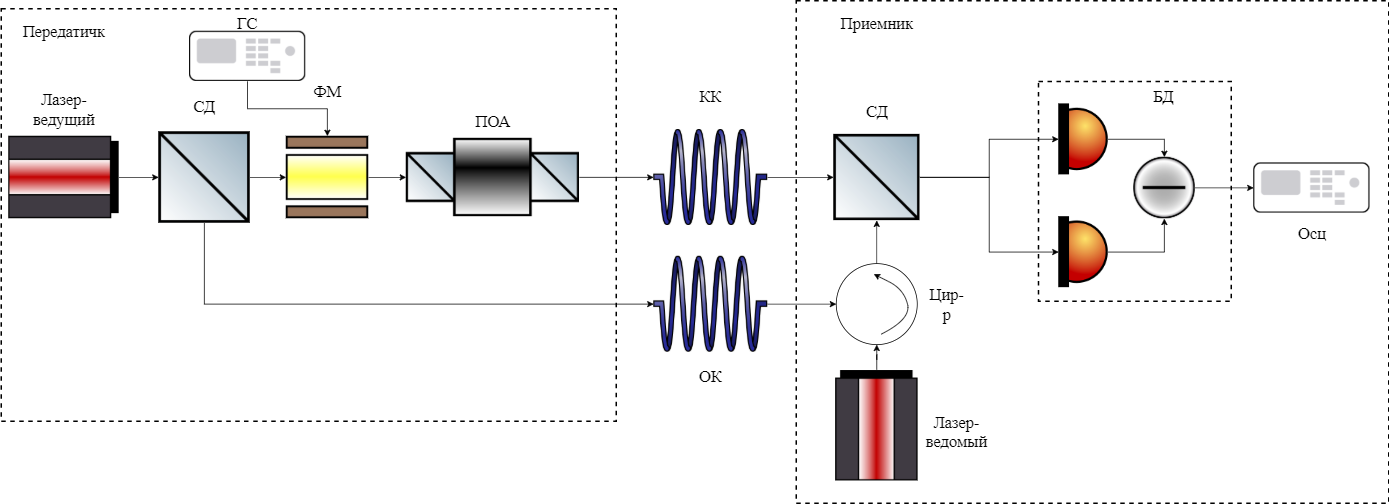
\includegraphics[width=\textwidth]{images/Схема с обратной связью.png}
    \caption{Схема эксперимента системы КРК с применением оптической инжекции. СД - светоделитель, ФМ - фазовый модулятор, ГС - генератор сигналов, ПОА - перестраиваемый оптический аттенюатор, КК - квантовый канал, ОК - открытый канал, Цир-р - циркулятор, БД - балансный детектор, Осц - осциллограф.}
    \label{fig:opt inj scheme}
\end{figure}
Данная система, оптическая схема которой изображена на рисунке \ref{fig:opt inj scheme}, работает следующим образом. На стороне передатчика излучение, сгенерированное лазером, разделяется на две части. Первая часть излучения попадает на фазовый модулятор Алисы, где происходит фазовая модуляция переменным электрическим сигналом, в который вносятся фазовые сдвиги для кодирования информации. В качестве кодирования может использоваться квадратурно-фазовая манипуляция или Quadrature Phase Shift Keying (QPSK) модуляция. Данный цифровой способ модуляции вносит фазовые сдвиги, соответствующие значениям 45\textdegree, 135\textdegree, 225\textdegree и 315\textdegree. Этим значениям фазовых сдвигов присваивается значение бит {00, 01, 10, 11}. В результате этого в спектре появляются три гармоники сигнала: $\omega$ - центральная частота лазера, $\omega$ - $\Omega$ - нижняя боковая частота  и $\omega$ + $\Omega$ - верхняя боковая частота, где $\Omega$ - частота модуляции. Излучение после модуляции описывается уравнением: 
\begin{align}
\label{eq:spectrum seed}
F_s(t) & = A_0 * \sin(\omega_0 t + \phi_0) + \frac{A_0 * m}{2} * (\sin((\omega_0 + \Omega)t + (\phi_0 + \phi (t))) - \notag \\
&- \frac{A_0 * m}{2} * (\sin((\omega_0 - \Omega)t + (\phi_0 - \phi (t)))),
\end{align}где $A_0$ - амплитуда исходного излучения,  $\omega$ - центральная частота лазера, $\omega$ - $\Omega$ - нижняя боковая частота  и $\omega$ + $\Omega$ - верхняя боковая частота, $\Omega$ - частота модуляции, $\phi_0$ - фаза исходного излучения, $\phi(t)$ - фаза модулирующего излучения, $t$ - время, $m$ - индекс модуляции. Индекс модуляции - величина отношения мощности на боковых частотах к мощности во всем спектре. Индекс модуляции пропорционален амплитуде модулирующего электрического сигнала.  Полученный спектр попадает на переменный оптический аттенюатор, затухание которого выстраивается таким образом, чтобы на боковых частотах была мощность, соответствующая заданному среднему числу фотонов, когда несущая может оставаться классической. Подготовленные квантовые состояния передаются в квантовый канал. 
Вторая же часть излучения проходит по отдельному волоконно-оптическому каналу на сторону приемника, где попадает в волоконно-оптический циркулятор так, что излучение заходит в резонатор ведомого лазера. 
Пришедшее излучение из квантового канала попадает на первый вход волоконного светоделителя с двумя входами и двумя выходами и коэффициентом деления 50:50. На второй же вход светоделителя попадает локальный осциллятор, представляющий собой излучение, сгенерированное отдельным лазером на приемной стороне. Благодаря наличию обратной связи в виде оптической инжекции, длина волны лазера на приемной стороне синхронизирована с длиной волны лазера Алисы. В результате ЛО и квантовые состояния интерферируют на светоделителе. В результате этой интерференции на выходе светоделителя появляются дополнительные гармоники на промежуточной частоте. Эти гармоники -  $\omega$ - $f$ - центральная частота лазера Алисы минус частота ЛО, ($\omega$ - $\Omega$) - $f$  - нижняя боковая частота минус частота ЛО   и ($\omega$ + $\Omega$) - $f$ - верхняя боковая частота минус частота ЛО, где $\Omega$ - частота модуляции, $\omega$ - частота лазера Алисы, $f$ - частота ЛО. 
\newline Результат этой интерференции регистрируется балансным детектором. Это устройство представляет собой два классических фотодиода, подключенных так, чтобы их токи вычитались. Такое подключение позволяет уменьшить собственные шумы детектора. После этого полученный ток попадает на фильтр низких частот для фильтрации постоянной составляющей. Полученный сигнал усиливается каскадом усилителей и передается на АЦП.  В результате на выходе балансного детектора формируется только один сигнал на частоте, совпадающей с частотой модуляции на стороне передатчика. Происходит это по той причине, что длина волны ЛО и лазера передатчика совпадают благодаря обратной связи в виде оптической инжекции. Таким образом на выходе детектора остается только составляющая ($\omega$ + $\Omega$) - $f$, а остальные преобразуются в постоянную составляющую, которые фильтруются. 
\begin{figure}
    \centering
    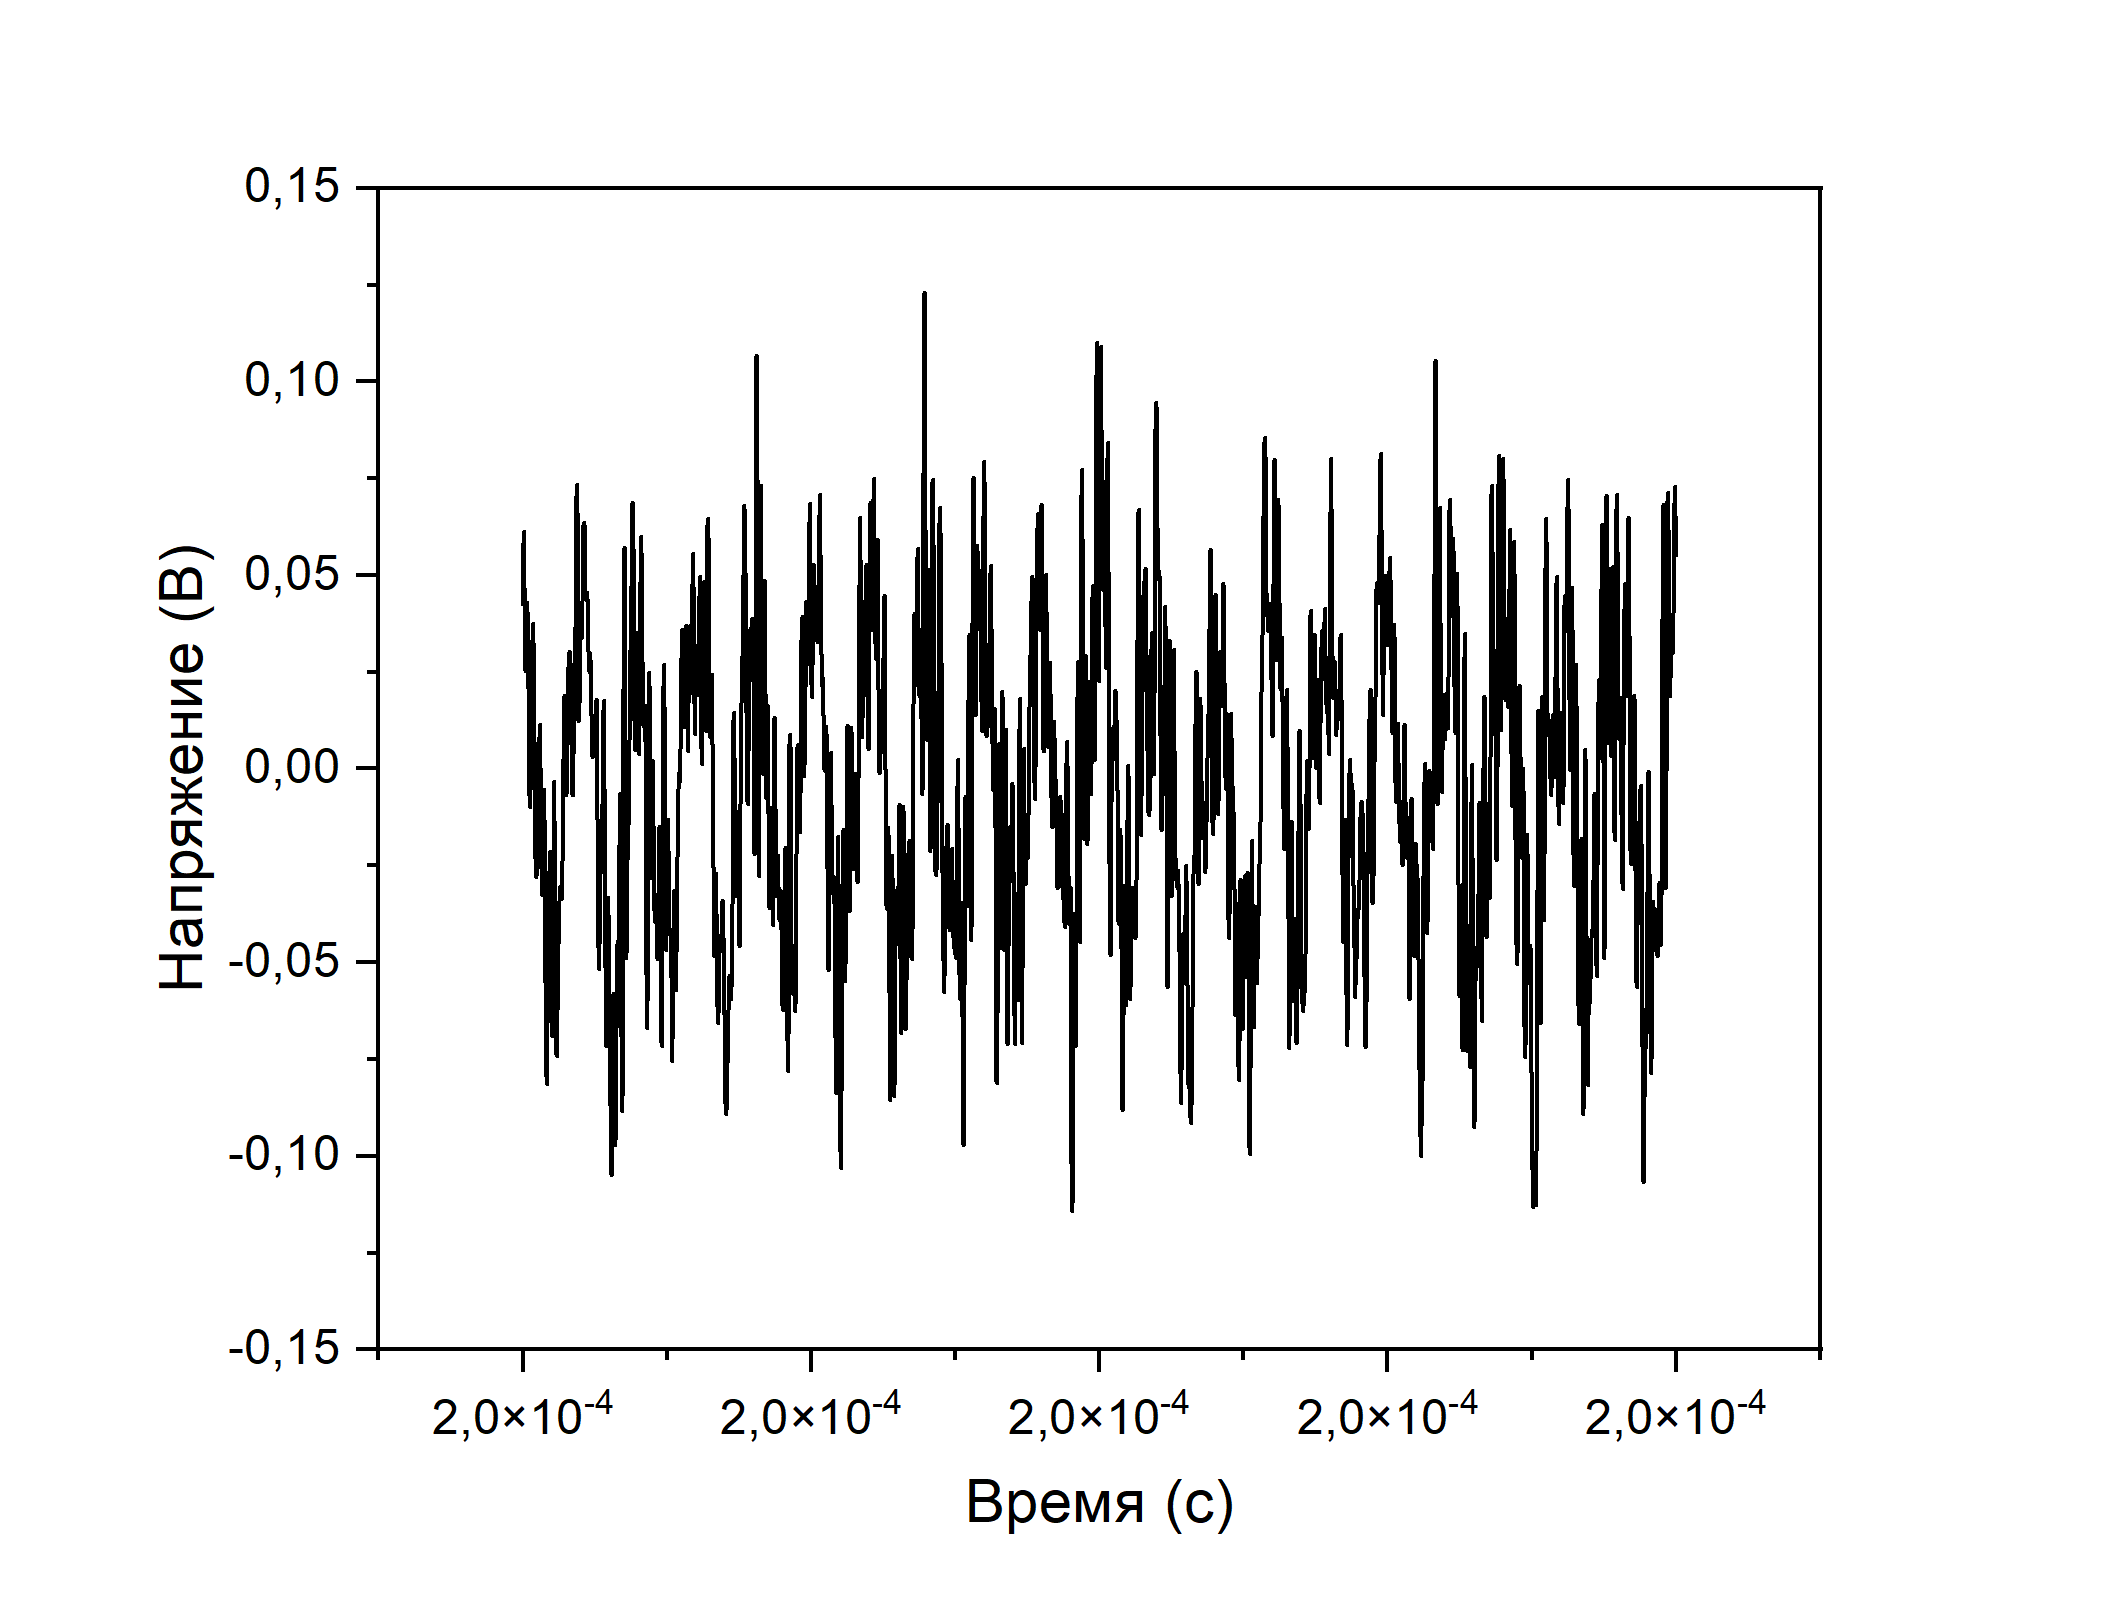
\includegraphics[width=\textwidth]{images/03.png}
    \caption{Зашумленный сигнал на выходе балансного детектора}
    \label{fig:noisy output inject}
\end{figure}
Полученное колебание на выходе балансного детектора несет в себе информацию о фазе, закодированную Алисой. Данный сигнал обрабатывается цифровыми методами обработки сигналов для извлечения значения фаз сигнала. 
\begin{figure}
    \centering
    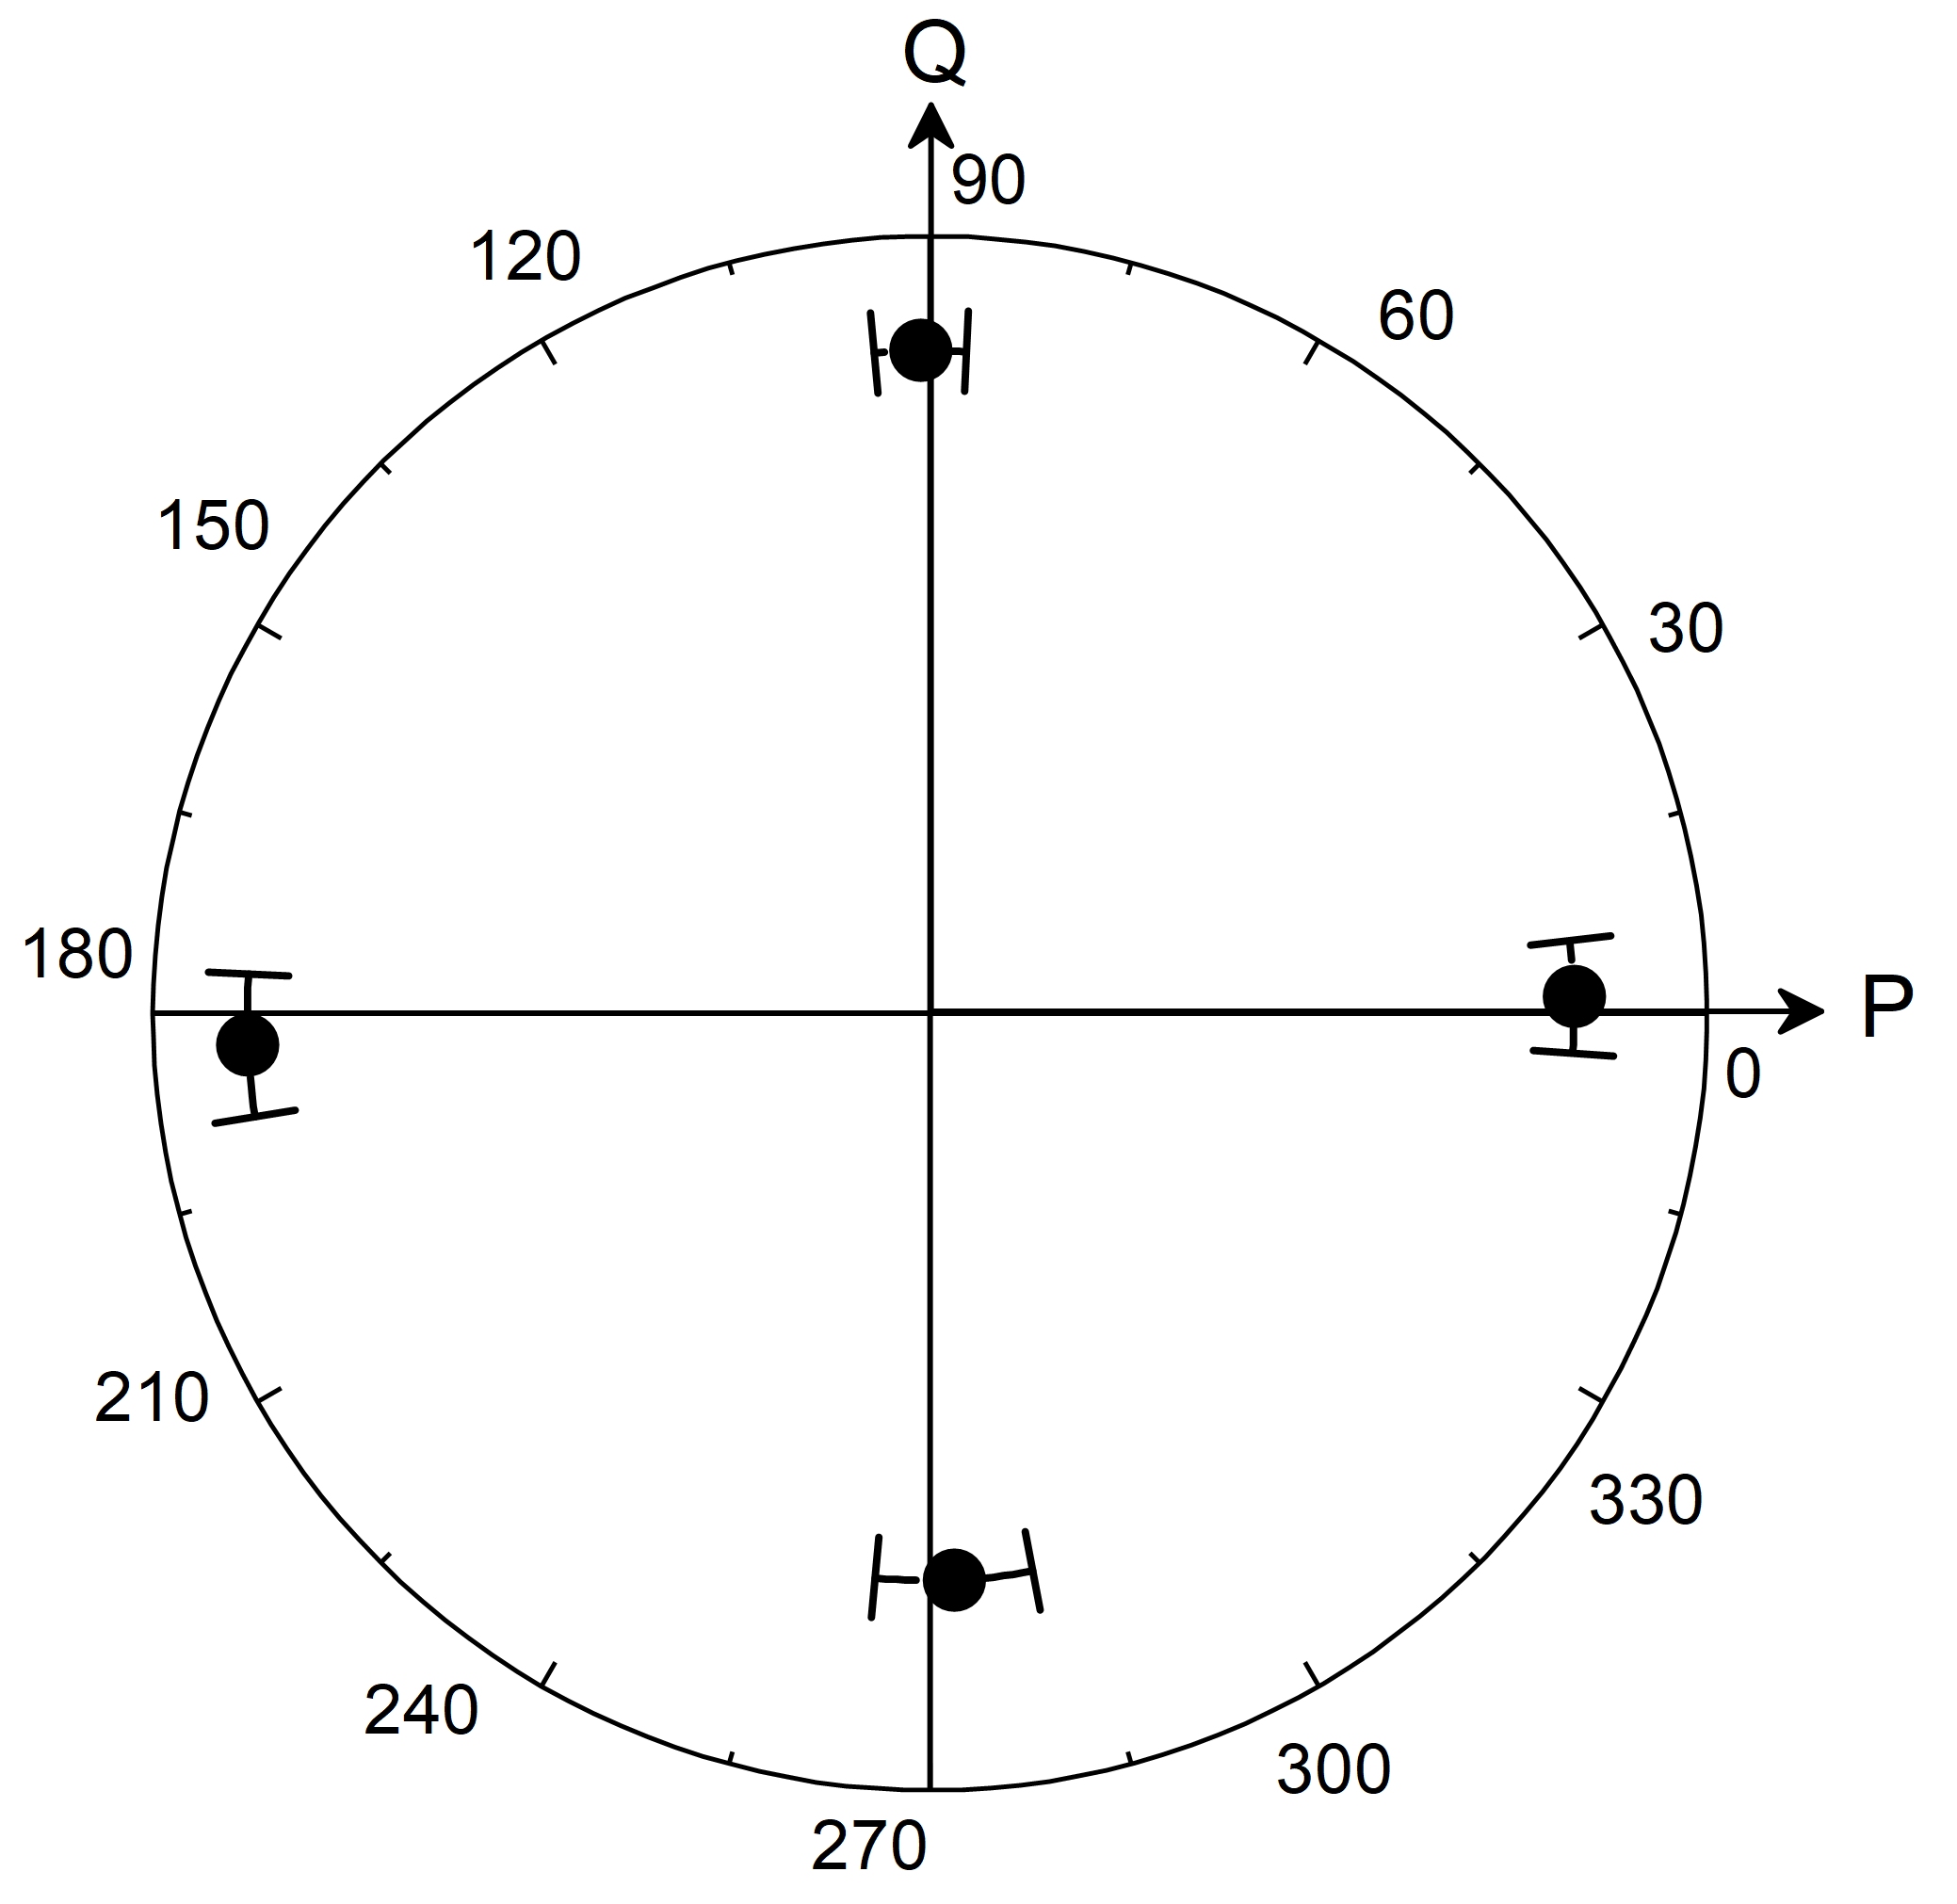
\includegraphics[width=0.8\textwidth]{new_iq_graph_het_true.png}
    \caption{Полученные значения фазы после цифровой обработки}
    \label{fig:phase meas ijnect}
\end{figure}

Полученная последовательность бит является сырым ключом. Полученный ключ просеивается. В полученном просеянном ключе оценивается квантовый коэффициент ошибок по битам (QBER), предварительно открыв часть ключа. И последним этапом происходит усиление секретности  с помощью HASH-функций.
\newline К плюсам данного метода реализации КРК можно отнести простоту системы, благодаря тому, что отсутствует активный выбор базиса в виде модулятора любого типа. Наличие обратной связи в виде оптической инжекции позволяет решить несколько проблем: стабилизация длины волны ЛО, что так же упрощает конечную систему, и уменьшает фазовые шумы, связанные со случайностью фазы лазерного излучения, сгенерированного разными источниками. Применение же гетеродинного метода приема позволяет использовать любой тип модуляции, что позволяет гибко настраивать протокол под различные задачи и оставляет задел на будущее для увеличения скорости выработки ключей.
\newline К недостаткам данной системы можно отнести необходимость дополнительного волоконно-оптического канала связи для организации обратной связи, что частично нивелируется тем, что реальные системы КРК встраиваются в уже существующие системы передачи данных, которые работают с технологией мультплексирования и сигнал оптической инжекции можно встроить в уже применяемые каналы, так как у него нет требований к уровню сторонних шумов. Второй же недостаток - это уязвимость к атаке засева лазера, который требует дополнительного изучения и контрмер. 
\newpage В \underline{третьей главе} рассматривается схема применения гетеродинного метода детектирования сигналов с двумя независимыми источниками сигналов для протокола квантовой коммуникации на боковых частотах. Особенностью данной системы является перенос квантовых состояний света на боковые частоты, которые появляются в спектре излучения. Основная реализация данного протокола предполагает использование дискретных переменных и детекторов одиночных фотонов на основе лавинных фотодиодов для регистрации сигналов. Однако этот протокол возможно адаптировать и для использования когерентных методов детектирования. 
\newline В данной работе предлагается использование гетеродинного метода детектирования сигналов для системы квантовой коммуникации на боковых частотах.
\begin{figure}
    \centering
    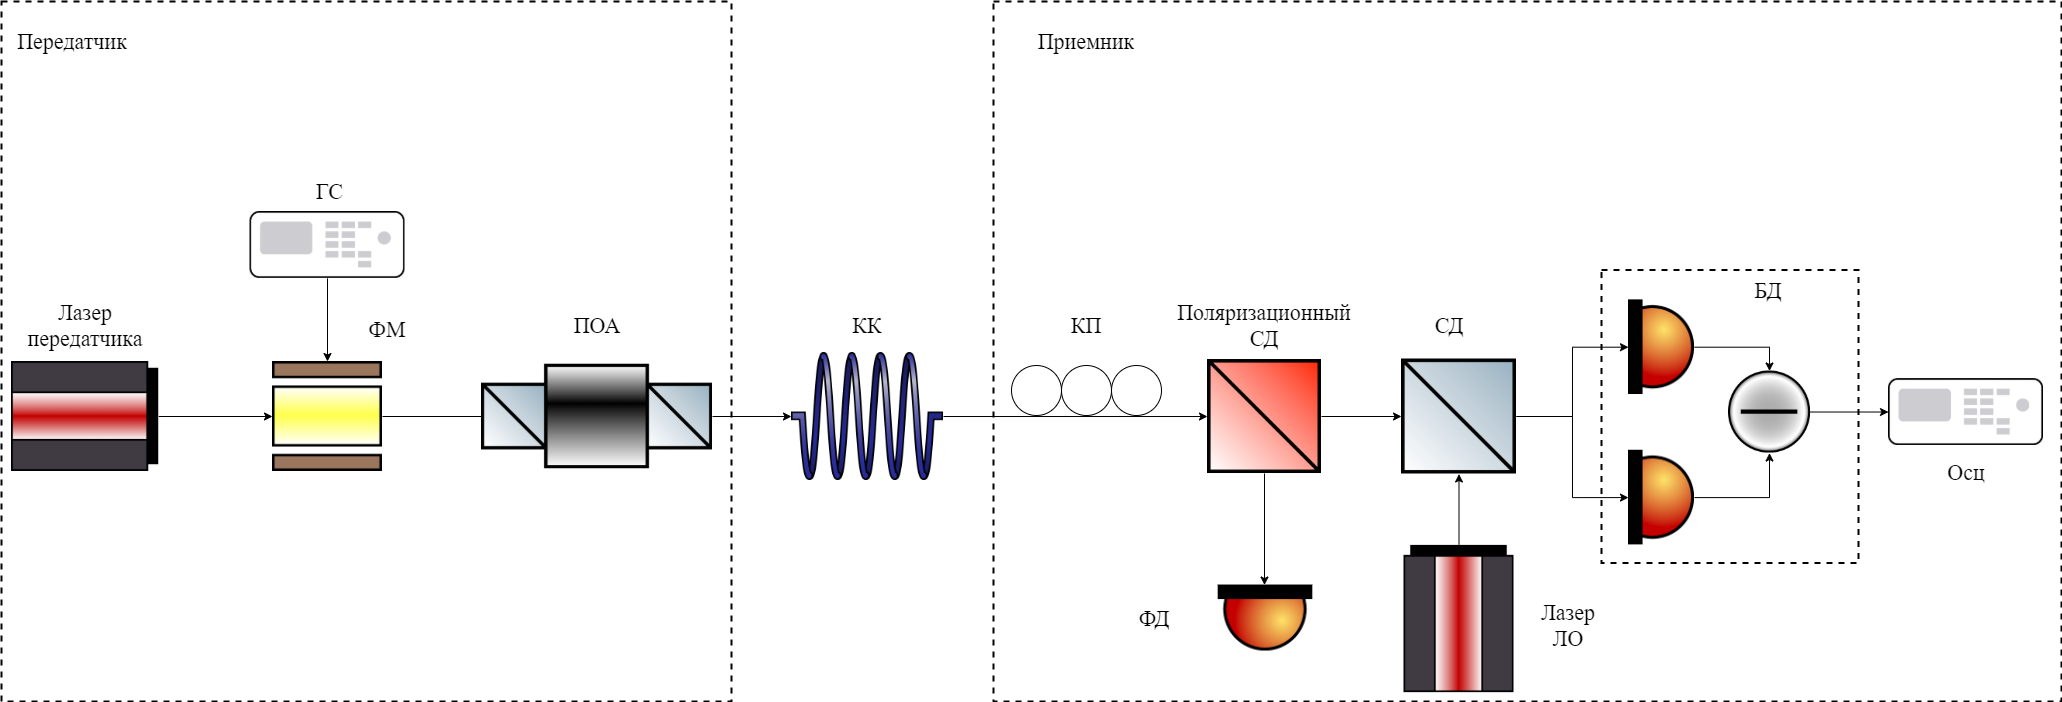
\includegraphics[width=\textwidth]{Гетеродин схема новая2 .png}
    \caption{Схема системы квантового распределения ключа на боковых частотах с независимым локальным осциллятором. СД - светоделитель, ФМ - фазовый модулятор, ГС - генератор сигналов, ПОА - перестраиваемый оптический аттенюатор, КК - квантовый канал, БД - балансный детектор, Осц - осциллограф.}
    \label{fig:het true scheme}
\end{figure}
Данная система работает следующим образом. Лазер на передающей стороне формирует когерентное излучение. Это излучение, пройдя необходимые пассивные элементы в виде оптических изоляторов, попадает на кристалл фазового модулятора. На электрический же вход фазового модулятора передается переменное напряжение на частоте модуляции. В это напряжение вносится фазовый сдвиг, который соответствует битам информации. Для примера в данной работе используется квадраратурно-фазовая манипуляция или quadrature phase-shift keying (QPSK). Значения фазовых сдвигов в таком случае это {45\textdegree, 135\textdegree, 225\textdegree и 315\textdegree} и этим фазовым сдвигам соответствуют следующие биты информации {00, 01, 10, 11}. В результате такой модуляции в спектре излучения после фазового модулятора появляются три гармоники, в двух из которых закодирована информация от передатчика. Подготовленное излучение ослабляется переменным аттенюатором для достижения уровня мощности на боковых частотах меньше 1 фотона в среднем. Полученные таким образом квантовые состояния передаются по волоконно-оптической линии связи на приемную сторону.  
\newline Переданный сигнал от Алисы после прохождения ВОЛС попадает на контроллер поляризации для компенсации искажений, внесенных прохождением через волокно. После этого установленный поляризационный светоделитель выделяет лишь нужную поляризацию и пропускает излучение с нужной поляризацией дальше. После этого квантовые состояния смешиваются с ЛО, сгенерированным отдельным лазером, на светоделителе с двумя входами и двумя выходами и коэффициентом деления 50:50. Эти сигналы интерферируют и в результате этой интерференции спектр излучения обогащается дополнительными гармониками. Эти гармоники появляются из-за того, что частоты ЛО и лазера Алисы не совпадают. Эти спектральные компоненты находятся на различных частотах - суммарная, разностная и комбинационные. Но с учетом ограниченности полосы пропускания балансного детектора, мы можем наблюдать на его выходе только гармоники на разностных частотах, которые в нее попадают. Суммарные и другие комбинационные частоты не попадают в полосу пропускания БД и регистрируются как постоянная составляющая, которая теряет всю информацию, закодированную в их фазы. Когда как гармонические колебания на разностной промежуточной частоте проходят усилительный каскад без изменений и сохраняют информацию, закодированную в фазу излучения Алисой. Таким образом происходит перенос спектра из оптической области в радиочастотную, где упрощается усиление и обработка сигналов. 
\begin{figure}
    \centering
    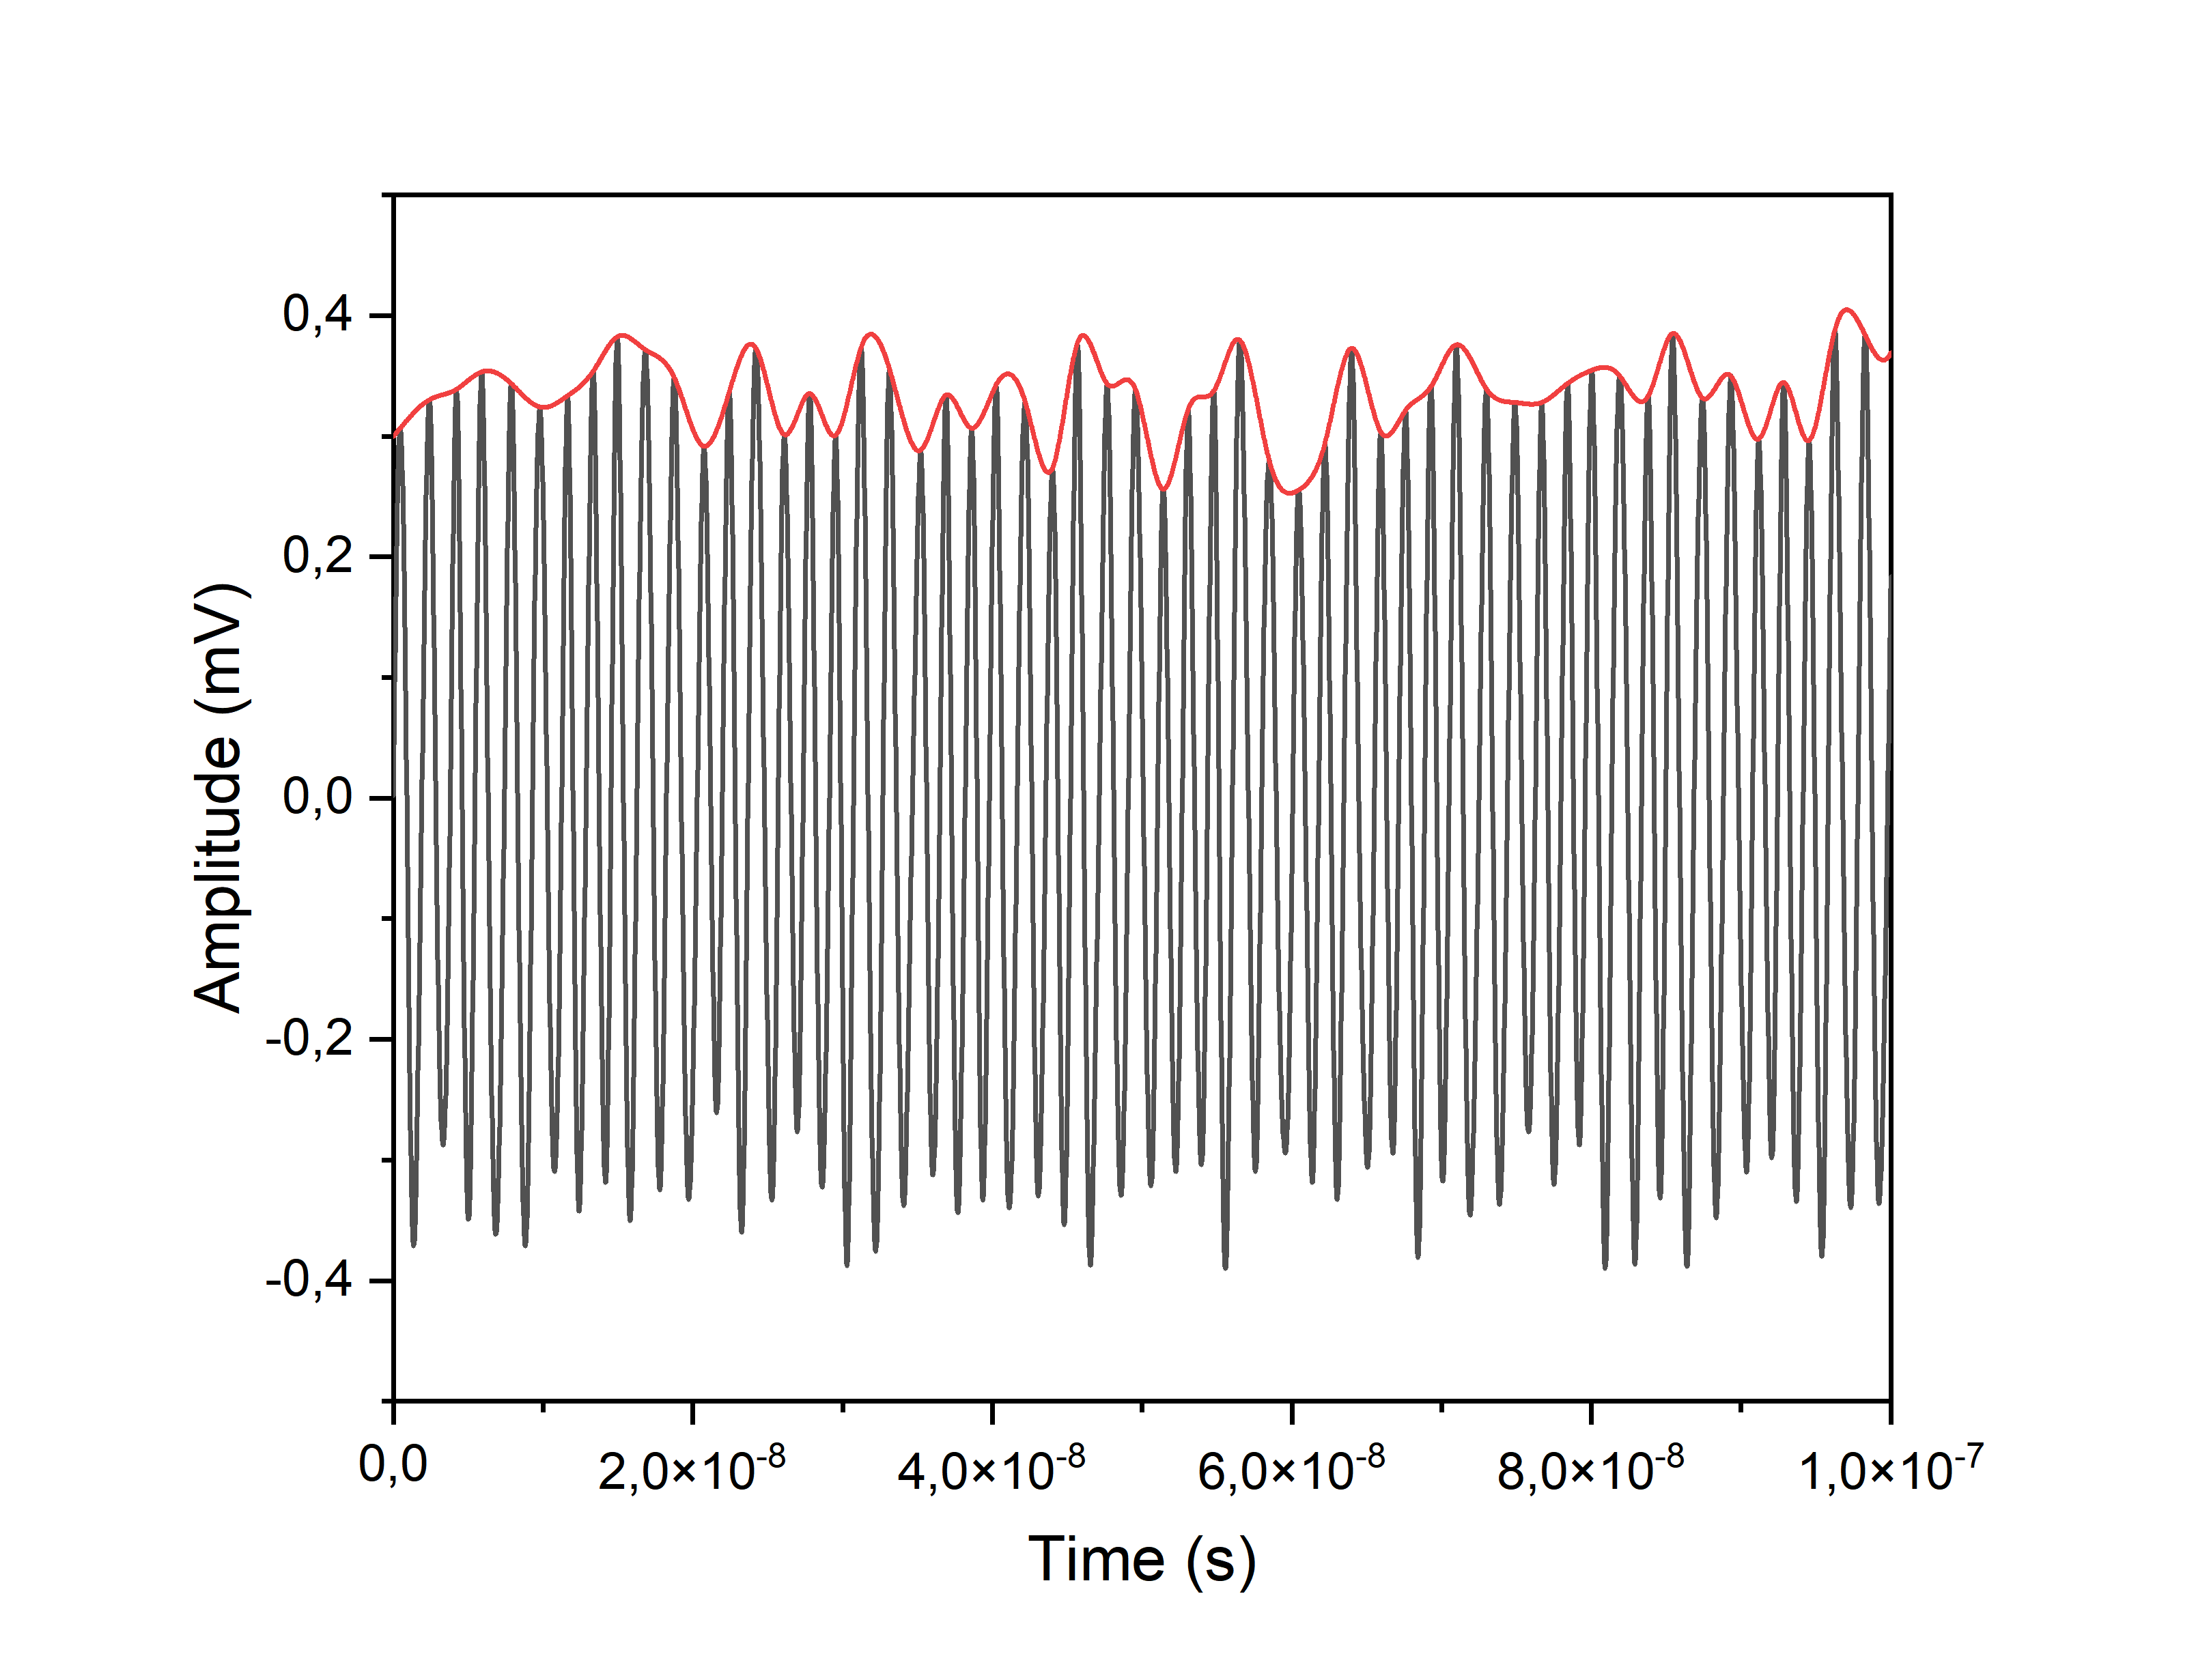
\includegraphics[width=\textwidth]{images/balanced output heterodyne.png}
    \caption{Сигнал на выходе балансного детектора после гетеродинного приема.}
    \label{fig:het time output}
\end{figure}
\newline Балансный детектор - это устройство, которое представляет собой два фотоприемных диода, подключенных так, чтобы их фототоки взаимно вычитались. После этого полученный сигнал подвергается фильтрации, чтобы исключить влияние постоянной составляющей фототока. После этого полученный сигнал попадает на каскад усилителей для увеличения его амплитуды. Наличие каскада усилителей ограничивает полосу пропускания всего устройства. Типичная ширина полосы пропускания может варьироваться от 100 МГц до 1.2 ГГц. Это ограничивает диапазон принимаемых частот и скорость выработки сырого ключа. 
\newline Полученный сигнал после усиления необходимо перевести в цифровую форму с помощью АЦП для его дальнейшей обработки. В качестве обработки могут применятся различные методы цифровой обработки сигналов, такие как Быстрое Преобразование Фурье или Преобразование Гильберта. В результате этой обработки из гармонического сигнала, полученного после АЦП, генерируются фазовые значения, которым соответствуют заданные значения бит, из которых формируется битовая последовательность, называемая сырым ключом. 
Однако использование ЛО на стороне приемника требует подстройки поляризации его и поляризации квантовых состояний для эффективной интерференции на приемнике. В рамках данной работы предлагается алгоритм контроля поляризации на основе Быстрого Преобразования Фурье. Суть данного алгоритма заключается в том, что при использовании поляризационного светоделителя частота модуляции, которая несет в себе информацию от передатчика, удваивается.
Это появление удвоенной частоты возможно отследить в частотной области. Для этого применяется следующий алгоритм 
\begin{enumerate}
    \item Применение БПФ к принятому сигналу
    \item Анализ спектрального состава сигнала
    \item Поворот поляризации сигнала до уничтожения гармоники на удвоенной частоте модуляции
    \item Дальнейший поворот поляризации сигнала до максимума гармоники на частоте модуляции
\end{enumerate}
В результате его работы возможна как подстройка поляризации за счет применения активного контроля поляризации, который будет использовать результат БПФ как обратную связь для подстройки поляризации. 
\begin{figure}
    \centering
    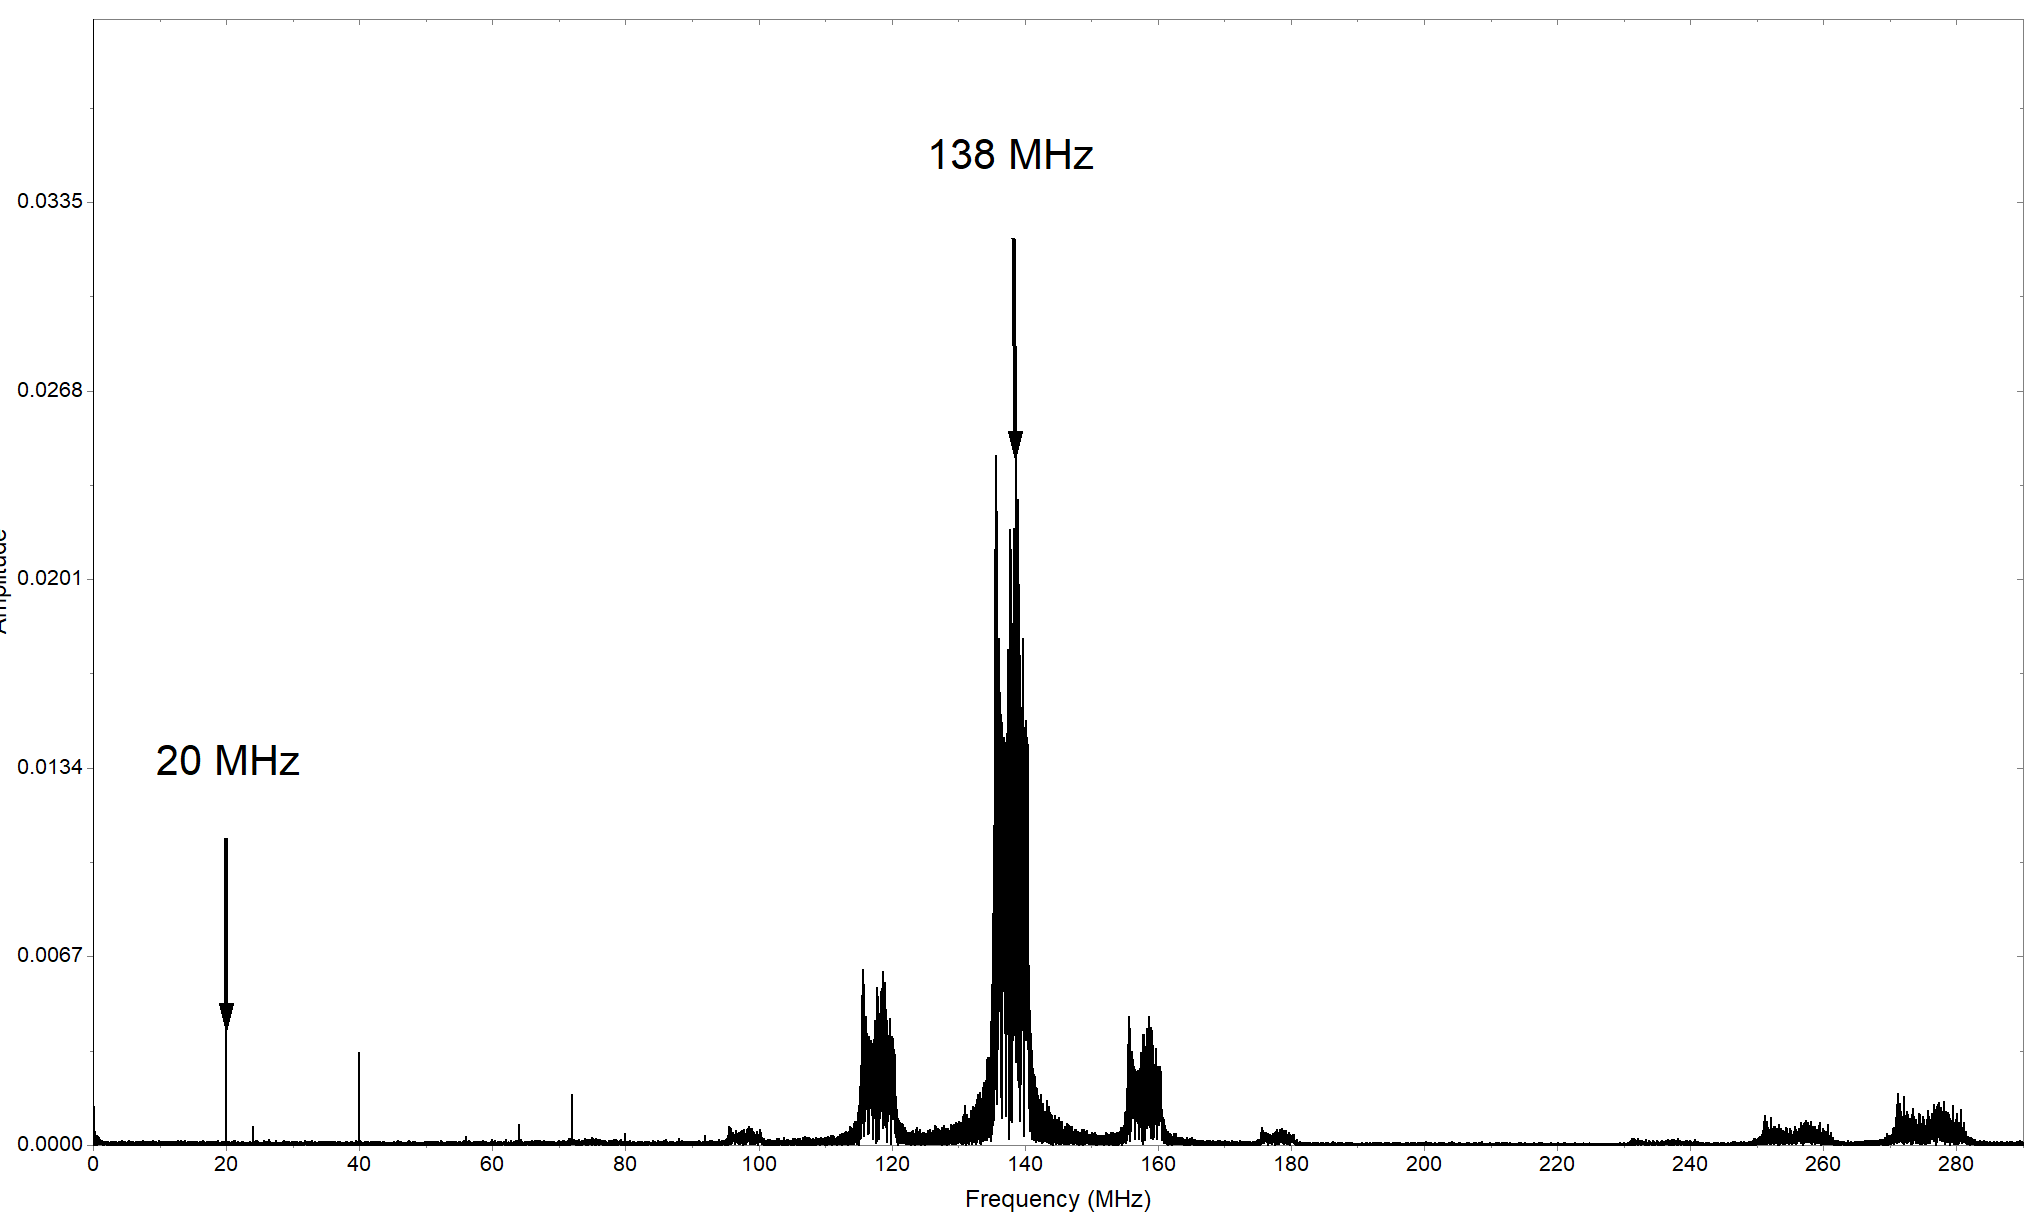
\includegraphics[width=\linewidth]{spectrum_het_true_ruin_pol.png}
    \caption{Спектр сигнала с искаженной поляризацией}
    \label{fig:ref ruin pol}
\end{figure}
\begin{figure}
    \centering
    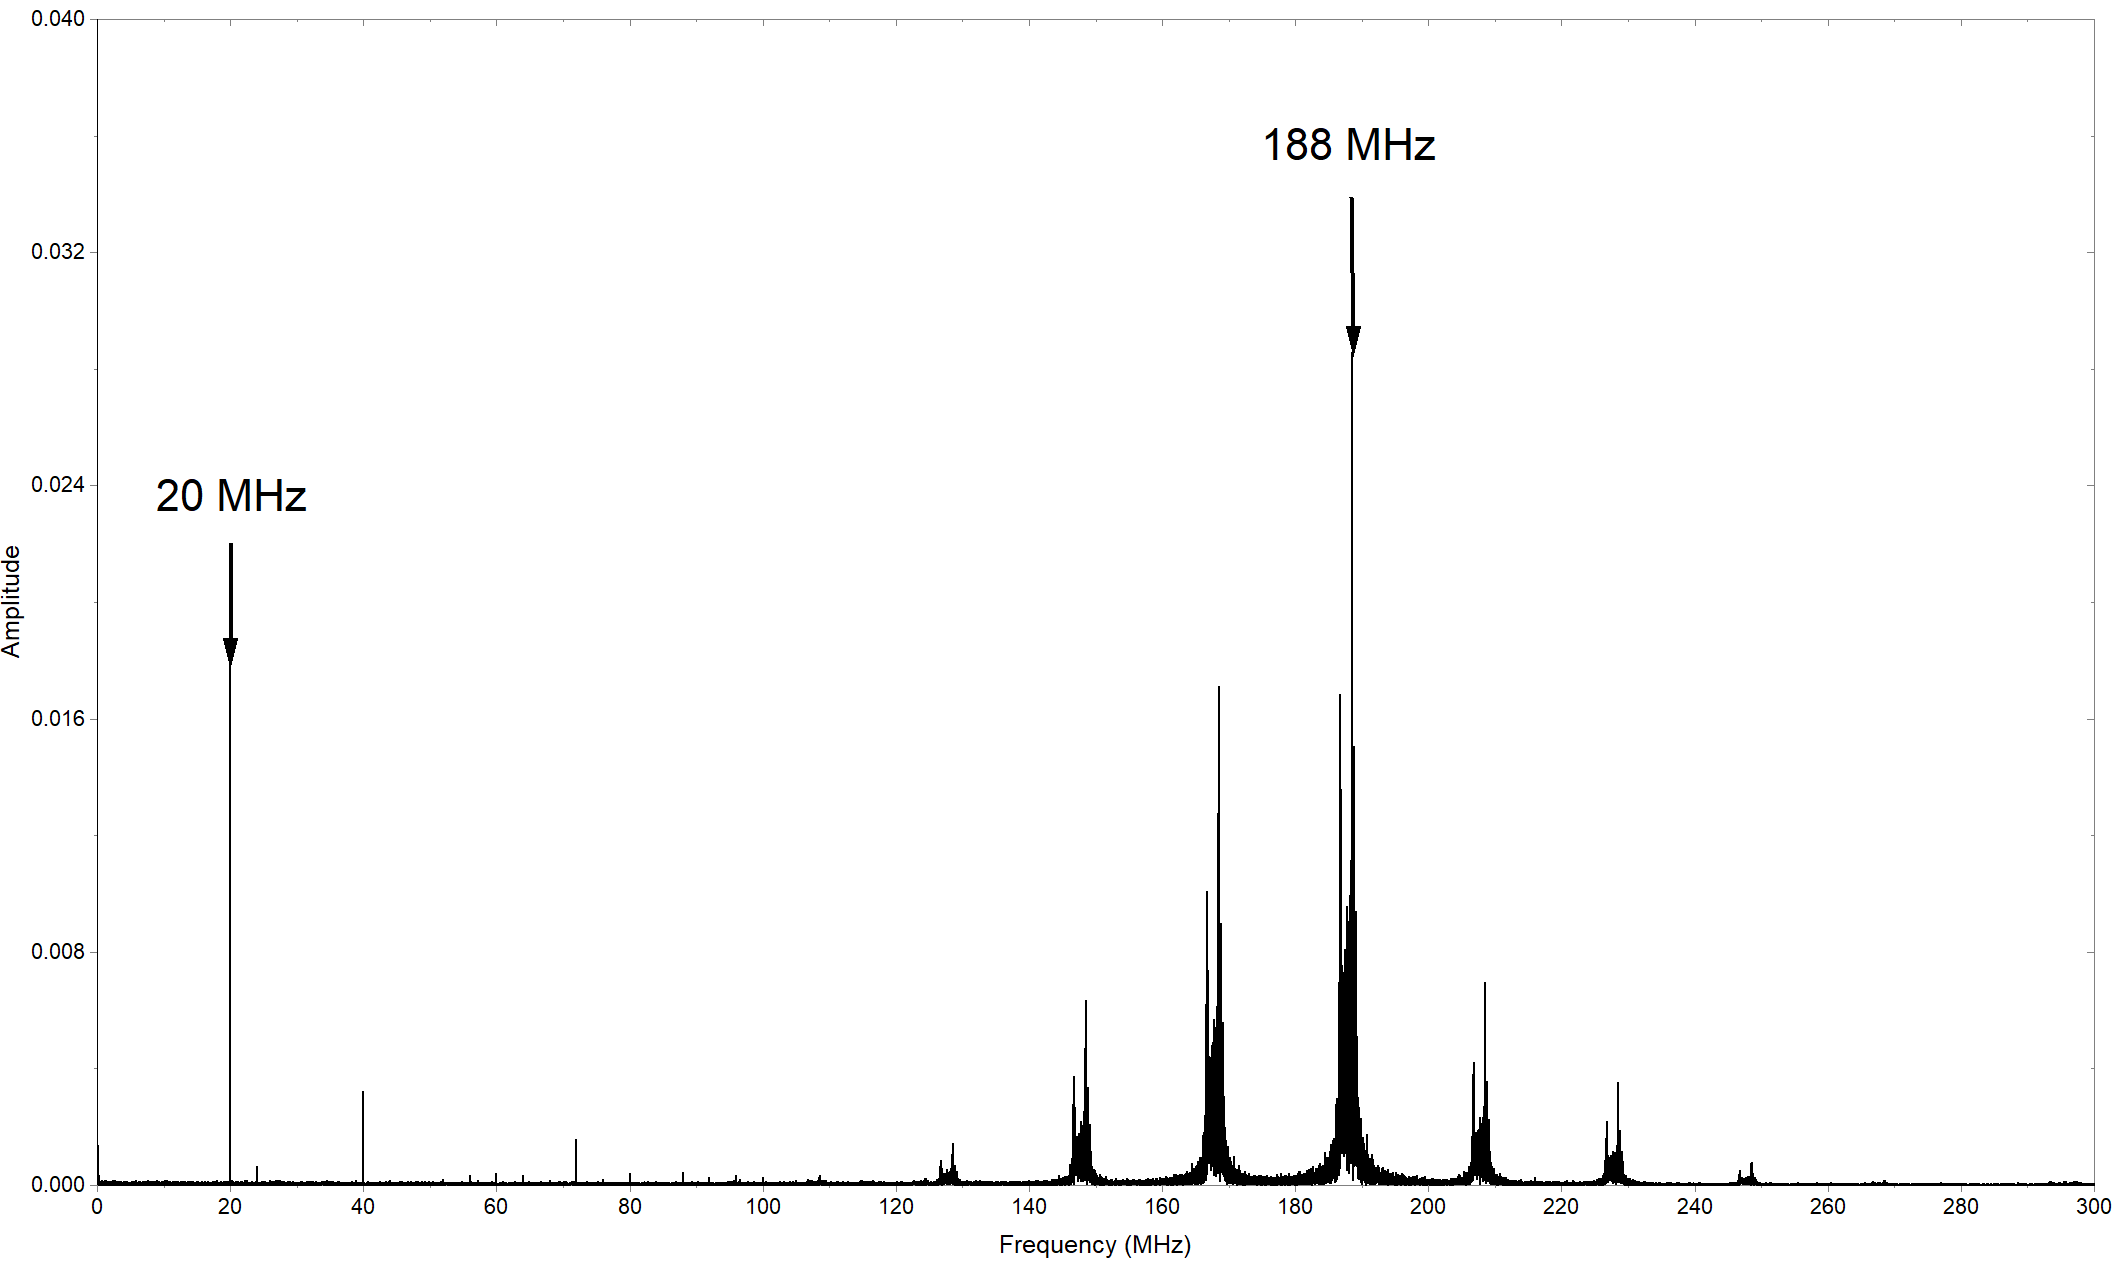
\includegraphics[width=\linewidth]{spectrum_het_true_norm_pol.png}
    \caption{Спектр сигнала с искаженной поляризацией}
    \label{fig:ref norm pol}
\end{figure}
На рисунке \ref{fig:ref ruin pol} изображен спектр информационного сигнала с искаженной поляризацией. Информация о наличии удвоенной частоте модуляции подается на контроллер поляризации, и он начинает свою работу до того момента, пока истинная частота модуляции не будет максимальной, а удвоенная частота модуляции - пропадет. Результат работы алгоритма изображен на рисунке \ref{fig:ref norm pol}. На спектре сигнала при нормальной поляризации не содержит гармоники на удвоенной частоте и при этом гармоника на частоте модуляции максимальна.
\newline К достоинствам данного метода можно отнести гибкость выбора протокола, так как перенос информации на промежуточную частоту позволяет анализировать практически любую модуляцию без необходимости внесения дополнительных элементов, например, фазового модулятора для выбора базиса. Использование двух независимых источников когерентного излучения позволяет не использовать системы обратной связи, которые требуют дополнительного оптического канала и открывают дополнительные возможности для злоумышленника. Генерация локального осциллятора на стороне приемника позволяет увеличить его мощность, по сравнению с протоколами, в которых ЛО передается по квантовому каналу, что позволяет уменьшить шумы, связанные с рассеянием в ВОЛС и увеличить соотношение сигнал/шум, что положительно влияет на скорость выработки бит. 
\newline Из недостатков же можно выделить необходимость подстройки частоты, так как два независимых генератора нуждаются в периодической подстройке частоты. Эта проблема решается особенностью протокола квантовой коммуникации на боковых частотах за счет того, что в спектре присутствует мощная несущая, которая так же сбивается с локальным осциллятором и переносится на промежуточную частоту. Анализируя эту частоту после обработки БПФ, можно подстраивать частоту ЛО для того, чтобы все сигналы попадали в полосу пропускания балансного детектора. Другим же недостатком является случайный фазовый шум из-за случайности процесса генерации лазерного излучения в двух независимых источниках. Данная проблема решается анализом фазы промежуточной частоты между локальным осциллятором и оптической несущей, полученной после фазовой модуляции Алисы. Этот сигнал будет содержать фазовый шум и ЛО, и лазера передатчика, который можно учесть в постобработке, сделав предварительную обработку цифровыми методами. 
\newpage \underline{Четвертая глава} посвящена изучению влияния излучения злоумышленника на длине волны 1310 нм на источник когерентного излучения на основе полупроводникового лазерного диода с распределенной обратной связью. Данная уязвимость в технической реализации получила название атака оптической накачкой. Данный тип атаки схож с атакой оптическим "засевом" (Laser Seeding) тем, что Ева инжектирует свое излучение в резонатор лазера на передатчике для изменений его характеристик. Однако есть существенное различие. В случае атаки "засевом" злоумышленник использует ту же или близкую длину волны к рабочей длине волны атакуемого лазера. В то время как в случае атаки оптической накачкой Ева использует длину волны лазера, отличающуюся на 50 и более нанометров от рабочей длины волны лазера Алисы. Эта особенность позволяет эффективнее обходить контрмеры с применением пассивных волоконно-оптических элементов в виде изоляторов. Их коэффициент изоляции имеет спектральную зависимость, что приводит к тому, что вносимая изоляция на длине волны 1310 нм существенно меньше, чем на длине волны 1550 нм. В результате злоумышленнику требуются меньшая зондирующая мощность, чтобы достичь необходимого эффекта. 
\newline Данная атака строится следующим образом. Злоумышленник устанавливает в разрыв волоконно-оптической линии связи волоконный циркулятор с тремя портами. В первый порт подключается зондирующий лазер Евы. Второй порт подключается в волоконно-оптическую линию связи в сторону отправителя, а третий порт - в сторону приемника. Таким образом излучение злоумышленника будет заходить в оптическую схему передатчика, а излучение Алисы будет проходить по волокну в сторону приемника без проблем. Излучение злоумышленника, проходя оптическую схему передатчика, претерпевает затухание, поэтому необходимо иметь достаточную мощность зондирующего излучения для внесения изменений в характеристики лазера. Прошедшее излучение попадает в кристалл лазера и поглощается в нем.
\begin{figure}
    \centering
    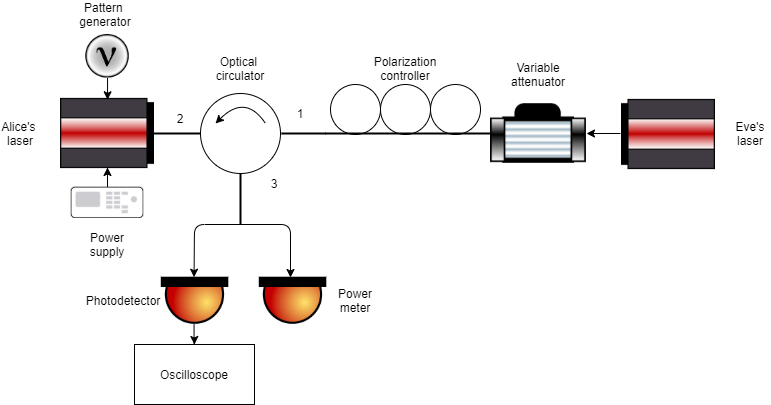
\includegraphics[width=0.75\textwidth]{images/1310 experiment.png}
    \caption{Схема эксперимента по засеиванию лазера. Alice's Laser -  Лазер Алисы, Pattern generator - генератор последовательности импульсов, Power Supply - лабораторный блок питания, optical circulator - оптический циркулятор, polarization controller - контроллер поляризации, varriable attenuator - перестраиваемый аттенюатор, Eve's laser - лазер злоумышленника, Photodetector - фотоприемник, power meter - измеритель мощности, Oscilloscope - осциллограф.}
    \label{fig:exper 1310 ref}
\end{figure}
Это приводит к тому, что создается дополнительная инверсия населенности, приводящая к смещению Ватт-Амперной характеристики лазера при неизменном токе накачки.
\begin{figure}
    \centering
    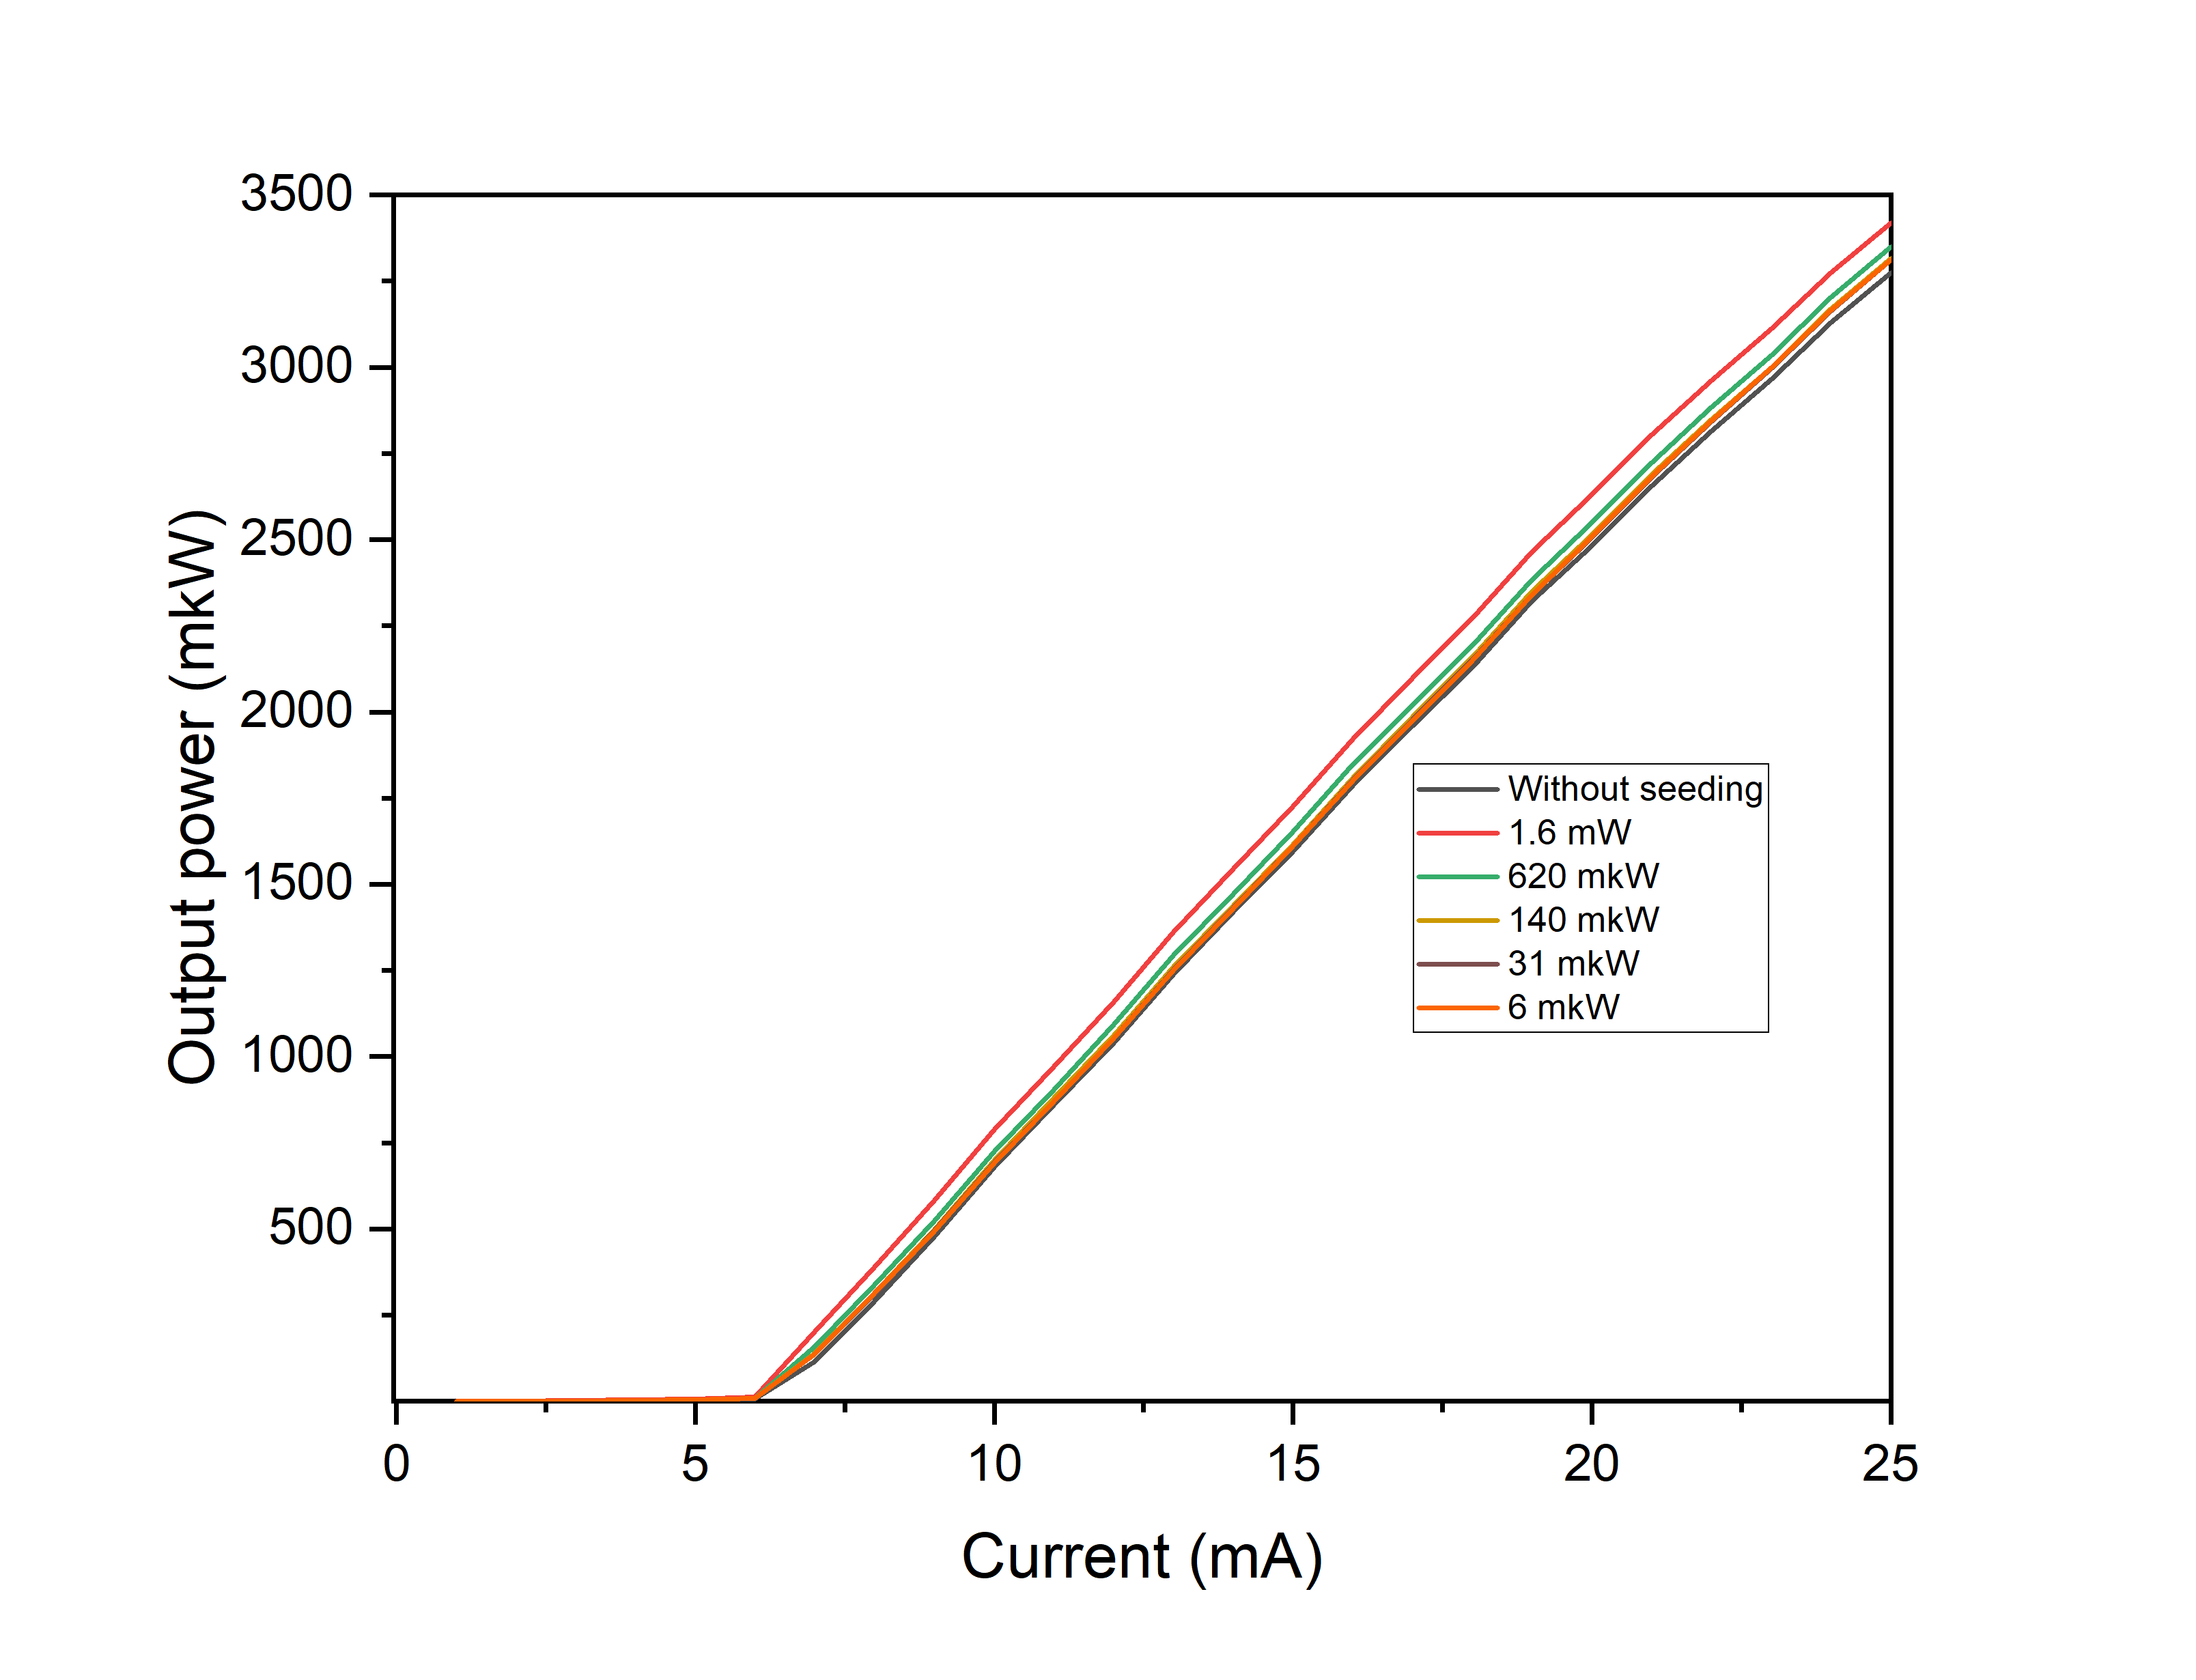
\includegraphics[width=0.75\textwidth]{images/ватт ампер для диссера.png}
    \caption{Изменение Ватт-Амперных характеристик под различными мощностями накачки на длине волны 1310 нм. Output power - выходная мощность в микроваттах, current - ток в миллиамперах}
    \label{fig:watt-amp ref}
\end{figure}
В результате этого калиброванный источник излучения на стороне передатчика начинает излучать большую мощность, чем предполагалось изначально. В итоге это приводит к тому, что выходное среднее число фотонов увеличивается, генерируется большее количество многофотонных состояний, что открывает возможности по реализации атаки с расщеплением числа фотонов. Этот же эффект проявляется в изменении формы импульса. Оптическая накачка увеличивает площадь импульса и, соответственно, его энергию, повышая как и среднее число фотонов в сигнальных импульсах, так и среднее число фотонов в состояния-ловушках в протоколе BB84 с состояниями-ловушками.
\begin{figure}
    \centering
    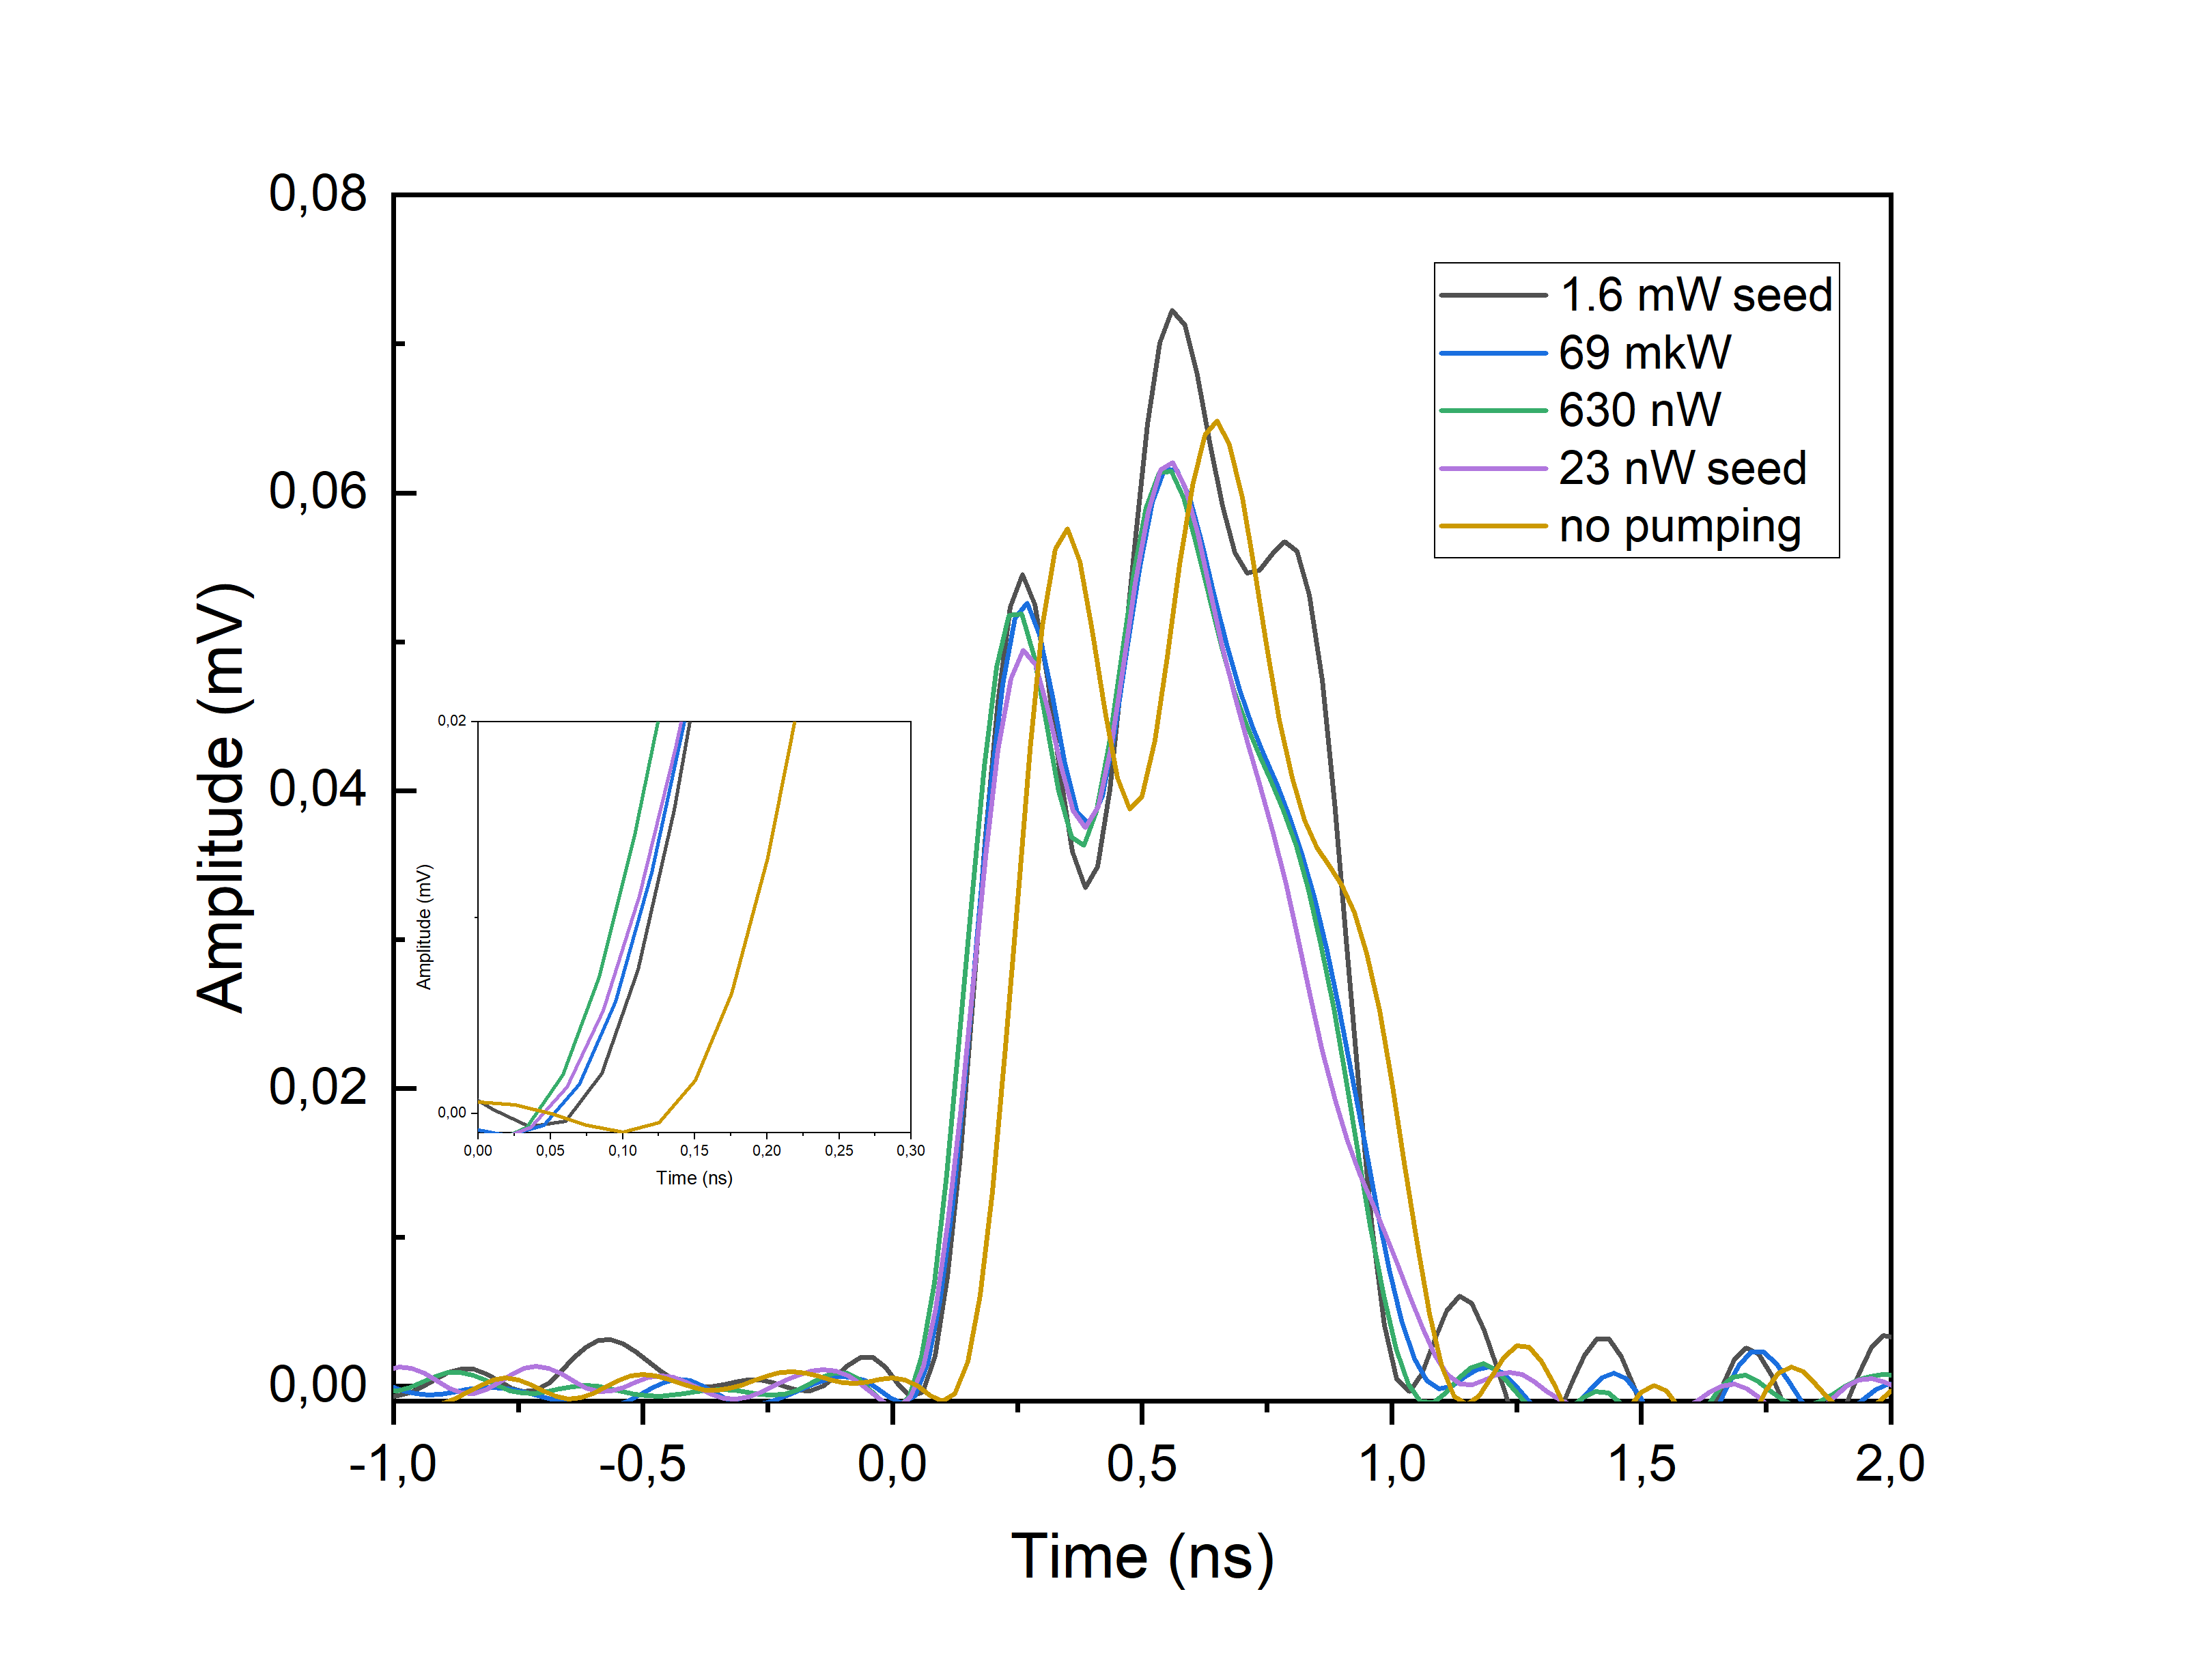
\includegraphics[width=0.75\textwidth]{images/Импульсы под действием 1310 для диссера.png}
    \caption{Измнение формы импульса под действием внешней оптической накачки на разных мощностях на длине волны 1310 нм. Amplitude - амплитуда в милливольтах, Time - время в наносекундах, seed - засеивание, pumping - накачка.}
    \label{fig:pulses 1310 ref}
\end{figure}
\newpage В рамках данной работы показана реализация атаки оптической накачкой на длине волны 1310 нм, которая приводит к увеличению выходной мощности лазера при неизменных токах накачки, увеличению площади импульса и повышению квантовой эффективности лазера. Данные эффекты создают условия для проведения других типов атак на систему КРК. В случае данной работы было показано, что зондирующей мощности в 200 мкВт достаточно для повышения квантовой эффективности на 1\%, продемонстрированно на графике \ref{fig:eff ref} и увеличения выходной мощности на 4\%. Была рассчитана минимально необходимая мощность для эффективной атаки злоумышленника на типичную оптическую схему передатчика, реализующую протокол BB84.
\begin{figure}
    \centering
    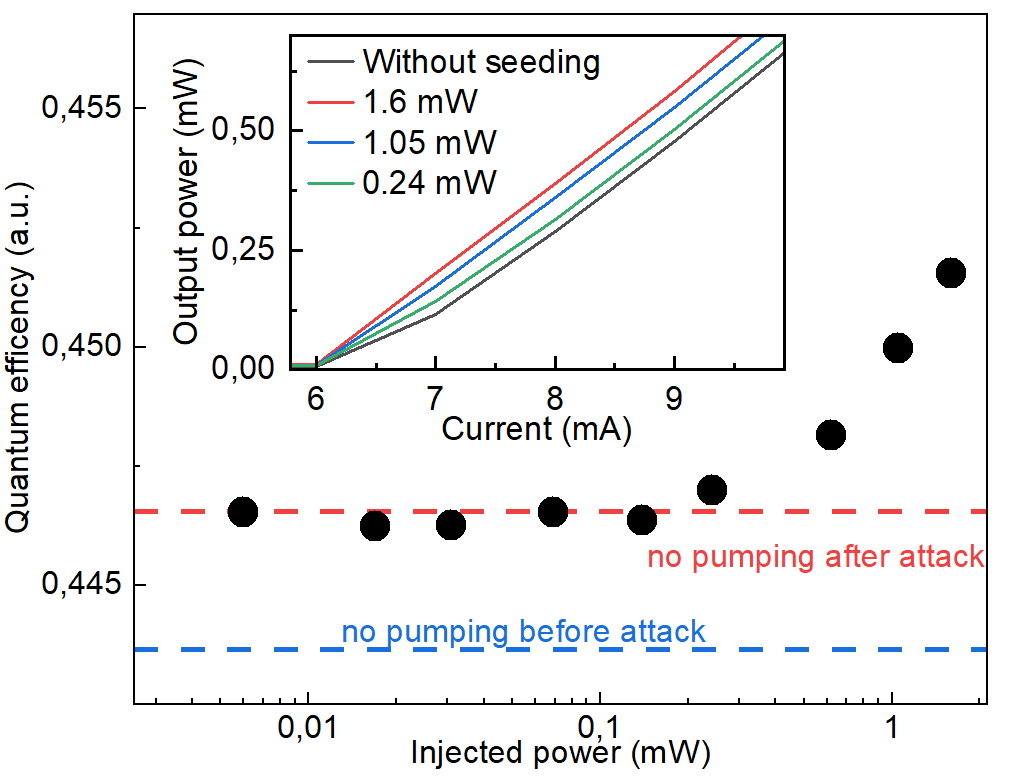
\includegraphics[width=0.7\textwidth]{images/Эффективность 1310.png}
    \caption{Изменение квантовой эффективности под действием внешнего излучения на длине волны 1310 нм. Quantum efficiency - квантовая эффективность в относительных единицах, Output power - выходная мощность в милливаттах, Injected power - введенная мощность в милливаттах, current - ток в миллиамперах, синяя пунктирная линия - значение квантовой эффективности до атаки, красная пунктирная линия - значение квантовой эффективности после атаки. }
    \label{fig:eff ref}
\end{figure}
\newpage Исследования, проводимые в \underline{шестой главе}, посвещены изучению влияния мощного когерентного излучения на источник лазерного излучения на основе оптической инжекции. Такие источники активно используются в системах квантовой коммуникации, реализующих протокол с недоверенным приемным узлом. Такие источники обладают улучшенными характеристиками стабильности амплитуды выходного сигнала, временной стабильностью длины волны и уменьшенным чирпом выходных импульсов за счет уменьшения влияния переходных процессов во время генерации. Эти особенности позволяют получать видность интерференции Хонг-Оу-Манделя близкой к теоретическому максимуму в 0.5. 
\newline Однако, для таких источников не были исследованы методы воздействия такие как атака "засевом" лазера. Для этого была собрана оптическая схема для проведения исследования влияния мощного лазерного излучения в диапазоне мощностей от 180 до 900 мВт. 
\begin{figure}
    \centering
    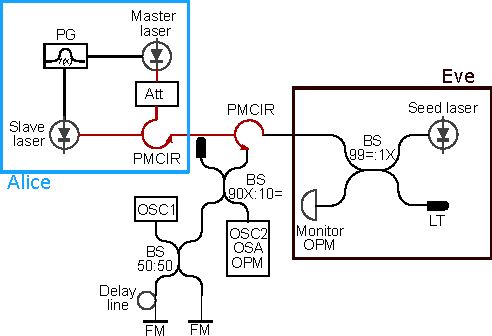
\includegraphics[width=0.9\textwidth]{images/setup_Faraday_Mirrors_final.pdf}
    \caption{Оптическая схема установки лазерного засеивания источника на основе оптической инжекции.}
    \label{fig:enter-label}
\end{figure}

В качестве источника были собраны два полупроводниковых лазера с распределенной обратной связью. Первый лазер - Agilecom WSLS-934010C4124-42 со встроенным изолятором, который использовался в качестве ведущего лазера для генерации опорного излучения. Второй же лазер представлял собой лазер Agilecom WSLS-934010C4124-82, аналогичный первому, но уже без встроенного изолятора. Это нужно для того, чтобы максимизировать количество излучения, вводимого в резонатор ведомого лазера. Эти два лазера подключены друг к другу через оптический циркулятор. Первый порт его подключен в ведущему лазеру, излучение из которого попадает на второй порт циркулятора, куда подключен ведомый лазер. Таким образом изучение из лазера-мастера попадает в резонатор ведомого лазера. Излучение ведомого лазера попадает на второй вход циркулятора и проходит на третий порт циркулятора. В качестве источника мощного лазерного излучения использовался лазер Gooch \& Housego AA1406-193300 и волоконный эрбиевый усилитель. Для введения его излучения использовался дополнительный циркулятор, первый порт которого подключается к выходу усилителя, второй к третьему порту первого циркулятора. Для исследования интерференции полученных импульсов был собран волоконный интерферометр Майкельсона. 
\newline В ходе работы были исследованы характеристики выходных импульсов под действием внешнего излучения. Исследовались следующие параметры: амплитуда выходных импульсов и их стабильность, выраженная в измерении стандартного отклонения, длительность импульсов и их стандартное отклонение, а также изучалась корреляция фазы полученных импульсов с помощью волоконного интерферометра Майкельсона. В ходе воздействия изменялось стандартное отклонение энергии выходных импульсов в диапазоне от 2 до 3.5 процентов при мощности лазера, атакующего в 900 мВт и при варьировании мощности лазера мастера. Результаты этих измерений приведены на рисунке \ref{fig:area MDI ref}
\begin{figure}
    \centering
    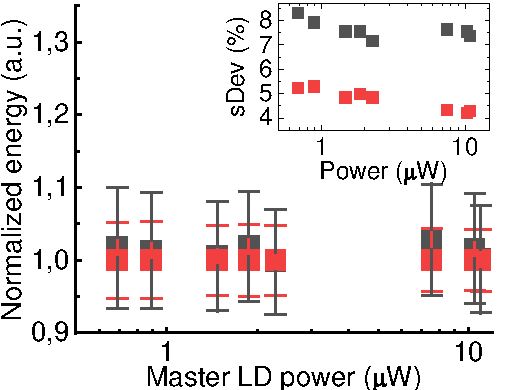
\includegraphics{images/area_under_attack.pdf}
    \caption{Изменение энергии импульса источника под действием внешнего излучения и без него в зависимости от мощности лазера-мастера.}
    \label{fig:area MDI ref}
\end{figure}
Данные результаты показывают, что Ева способна увеличивать нестабильность выходной мощности для увеличения среднего числа фотонах в импульсе. Длительность импульса так же изменяется под действием внешнего излучения, изображенном на рисунке \ref{fig:duration ref}. Под внешним воздействием дрожание импульса возрастает на 2\%.  Существующие работы показывают, что даже незначительные отклонения в длительности импульса существенно снижают дальность распределения секретного ключа. 
\begin{figure}
    \centering
    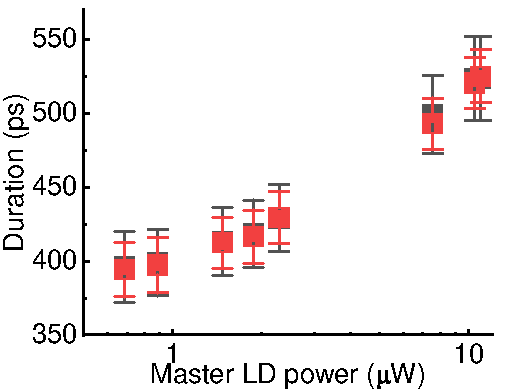
\includegraphics{images/duration_change.pdf}
    \caption{Измененение длительности импульса под действием внешнего излучения}
    \label{fig:duration ref}
\end{figure}
\newline Для разработки контрмеры необходимо рассчитать необходимый коэффициент изоляции для худшего сценария, когда злоумышленник использует максимально доступную ему мощность. В непрерывном режиме эта величина составляет 2 Ватта. Эту величину необходимо ослабить до значения меньше -35 дБм. Благодаря использованию в составе схемы волоконно-оптического циркулятора, величина изоляции уже составляет 50 дБ.  Для расчёта необходимого значения аттенюации используется формула
\begin{equation}
\label{eq:isolation}
    \alpha = P_a - P_{req} - \beta
\end{equation}, где $\alpha$ - величина изоляции, которую необходимо внести, $P_a$ - величина зондирующей мощности в дБм, $P_{req}$ - мощность, до которой требуется ослабить входное излучение, $\beta$ - величина изоляции, которая уже реализована в схеме, в дБ. 
Подставим в \ref{eq:isolation} значения в 33 дБм мощности, что соответствует 2 Ваттам мощности и 50 дБ изоляции. В результате значение изоляции, необходимое для ослабления 2 Ватт до -35 дБм, равняется 18 дБ. Для обеспечения безопасности данного источника достаточно установить волоконный изолятор, типичная величина изоляции которого равна 30 дБ. Это перекроет весь допустимый диапазон зондирующих мощностей. 
\newline Полученные результаты демонстрируют стойкость предложенного источника когерентного излучения ко внешним воздействиям. Для изменения его характеристик злоумышленнику необходимо работать на мощностях, близких к мощностям, запускающих искру в волоконно-оптических линиях связи, что несет для него повышенные риски быть обнаруженным. А протоколы, основанные на протоколе с использованием недоверенного приемного узла обезопашены не только от атак злоумышленника на приемные узлы в виде детекторов одиночных фотонов, но так и от атак на источники одиночных фотонов.
